%%% File encoding: UTF-8
%%% äöüÄÖÜß  <-- keine deutschen Umlaute hier? UTF-faehigen Editor verwenden!

%%% Magic Comments zum Setzen der korrekten Parameter in kompatiblen IDEs
% !TeX encoding = utf8
% !TeX program = pdflatex 
% !TeX spellcheck = de_DE
% !BIB program = biber

\documentclass[bachelor,german]{hgbthesis}
% Zulässige Optionen in [..]: 
%   Typ der Arbeit: diploma, master (default), bachelor, internship 
%   Hauptsprache: german (default), english
%%%----------------------------------------------------------

\RequirePackage[utf8]{inputenc}		% bei der Verw. von lualatex oder xelatex entfernen!

\usepackage[printonlyused]{acronym}
\usepackage{float} 
\graphicspath{{images/}}    % Verzeichnis mit Bildern und Grafiken
\logofile{logo}				% Logo-Datei = images/logo.pdf (\logofile{}, wenn kein Logo gewünscht)
\bibliography{references}  	% Biblatex-Literaturdatei (references.bib)

%%%----------------------------------------------------------
% Angaben für die Titelei (Titelseite, Erklärung etc.)
%%%----------------------------------------------------------

%%% Einträge für ALLE Arbeiten: -----------------------------
\title{Industrielle Cloud Applikationen in Industrie 4.0 mit Siemens MindSphere}
\author{Dipl.-Ing. Elisabeth \ Egger}
\programname{Software Engineering }
\placeofstudy{Hagenberg}
\dateofsubmission{2018}{01}{25}	% {YYYY}{MM}{DD}

%%% Zusätzlich für eine Bachelorarbeit: ---------------------
\thesisnumber{S1510307005-A}   % Stud-ID, z.B. 1310238045-A  
% (A = 1. Bachelorarbeit)
\semester{Wintersemester 2017/2018} 
\coursetitle{???} 
\advisor{Susanne Schaller, \ MMSc}

%%% Restriktive Lizenformel anstatt CC (nur für Typ master) -
%\strictlicense

%%%----------------------------------------------------------
\begin{document}
%%%----------------------------------------------------------

%%%----------------------------------------------------------
\frontmatter                    % Titelei (röm. Seitenzahlen)
%%%----------------------------------------------------------

\maketitle
\tableofcontents

%\chapter{Vorwort} 	% engl. Preface


Dies ist \textbf{Version \hgbthesisDate} der \latex-Dokumentenvorlage für 
verschiedene Abschlussarbeiten an der Fakultät für Informatik, Kommunikation
und Medien der FH Oberösterreich in Hagenberg, die mittlerweile auch 
an anderen Hochschulen im In- und Ausland gerne verwendet wird.

Das Dokument entstand ursprünglich auf Anfragen von Studierenden,
nachdem im Studienjahr 2000/01 erstmals ein offizieller
\latex-Grundkurs im Studiengang Medientechnik und -design an der
FH Hagenberg angeboten wurde. Eigentlich war die Idee, die bereits
bestehende \emph{Word}-Vorlage für Diplomarbeiten "`einfach"' in
\latex\ zu übersetzen und dazu eventuell einige spezielle
Ergänzungen einzubauen. Das erwies sich rasch als wenig
zielführend, da \latex, \va was den Umgang mit Literatur und
Grafiken anbelangt, doch eine wesentlich andere Arbeitsweise
verlangt. Das Ergebnis ist -- von Grund auf neu geschrieben und
wesentlich umfangreicher als das vorherige Dokument --
letztendlich eine Anleitung für das Schreiben mit \latex, ergänzt
mit einigen speziellen (mittlerweile entfernten) Hinweisen für \emph{Word}-Benutzer.
Technische Details zur aktuellen Version finden sich in Anhang \ref{app:TechnischeInfos}.

Während dieses Dokument anfangs ausschließlich für die Erstellung
von Diplomarbeiten gedacht war, sind nunmehr auch  
\emph{Masterarbeiten}, \emph{Bachelor\-arbeiten} und \emph{Praktikumsberichte} 
abgedeckt, wobei die Unterschiede bewusst gering gehalten wurden.

Bei der Zusammenstellung dieser Vorlage wurde versucht, mit der
Basisfunktionalität von \latex das Auslangen zu finden und -- soweit möglich --
auf zusätzliche Pakete zu verzichten. Das ist nur zum Teil gelungen;
tat\-säch\-lich ist eine Reihe von ergänzenden "`Paketen"' notwendig, wobei jedoch
nur auf gängige Erweiterungen zurückgegriffen wurde.
Selbstverständlich gibt es darüber hinaus eine Vielzahl weiterer Pakete,
die für weitere Verbesserungen und Finessen nützlich sein können. Damit kann
sich aber jeder selbst beschäftigen, sobald das notwendige Selbstvertrauen und
genügend Zeit zum Experimentieren vorhanden sind.
Eine Vielzahl von Details und Tricks sind zwar in diesem Dokument nicht explizit
angeführt, können aber im zugehörigen Quelltext jederzeit ausgeforscht
werden.

Zahlreiche KollegInnen haben durch sorgfältiges Korrekturlesen und
konstruktive Verbesserungsvorschläge wertvolle Unterstützung
geliefert. Speziell bedanken möchte ich mich bei Heinz Dobler für
die konsequente Verbesserung meines "`Computer Slangs"', bei
Elisabeth Mitterbauer für das bewährte orthographische Auge und
bei Wolfgang Hochleitner für die Tests unter Mac~OS.

Die Verwendung dieser Vorlage ist jedermann freigestellt und an
keinerlei Erwähnung gebunden. Allerdings -- wer sie als Grundlage
seiner eigenen Arbeit verwenden möchte, sollte nicht einfach
("`ung'schaut"') darauf los werken, sondern zumindest die
wichtigsten Teile des Dokuments \emph{lesen} und nach Möglichkeit
auch beherzigen. Die Erfahrung zeigt, dass dies die Qualität der
Ergebnisse deutlich zu steigern vermag.

Der Quelltext zu diesem Dokument sowie das zugehörige
\latex-Paket sind in der jeweils aktuellen Version online
verfügbar unter
%
\begin{itemize}
\item[]\url{https://github.com/Digital-Media/HagenbergThesis}.
\end{itemize}
%
Trotz großer Mühe enthält dieses Dokument zweifellos Fehler und Unzulänglichkeiten
-- Kommentare, Verbesserungsvorschläge und passende Ergänzungen
sind daher stets willkommen, am einfachsten per E-Mail direkt an mich:
\begin{itemize}
\item[]%

Dr.\ Wilhelm Burger, Department für Digitale Medien,\newline
Fachhochschule Oberösterreich, Campus Hagenberg (Österreich)\newline
\nolinkurl{wilhelm.burger@fh-hagenberg.at}
\end{itemize}

\noindent
Übrigens, hier im Vorwort (das bei Diplom- und Masterarbeiten üblich, bei Bachelorarbeiten 
aber entbehrlich ist) kann kurz auf die Entstehung des Dokuments eingegangen werden.
Hier ist auch der Platz für allfällige Danksagungen (\zB an den Betreuer, 
den Begutachter, die Familie, den Hund, \ldots), Widmungen und philosophische 
Anmerkungen. Das sollte allerdings auch nicht übertrieben werden und sich auf 
einen Umfang von maximal zwei Seiten beschränken.




 % Optional. Ggf. weglassen
\chapter{Kurzfassung}


TODO ÜBERARBEITUNG
\vspace{\baselineskip}
\vspace{\baselineskip}


Die Fa. Siemens AG bietet mit MindSphere eine neue Plattform für den Einsatz von Industrial Internet of Things und Cloud-Computing an. Industrielle Anlagen können so auf einfache Weise Daten in eine Cloud-Umgebung liefern. 

Im Detail geschieht dies durch Sensoren, welche Daten über speicherprogrammierbare Steuerungen sammeln und diese mit Hilfe von MindConnect Modulen an die Cloud MindSphere transferieren, wo diese gespeichert werden. 

Von diesem Zeitpunkt an stehen die Daten für diverse Auswertungen über die MindSphere API jederzeit zur Verfügung. 

Am Standort Siemens Graz soll nun evaluiert werden, wie sich die Plattform MindSphere für die Umsetzung von Kundenprojekten eignet. 

Ziel dieser Bachelorarbeit ist es, zu zeigen, wie eine Umsetzung einer MindSphere Applikation funktionieren kann und zu prüfen, welche Probleme dabei derzeit noch auftreten. Konkret soll ein einfaches Beispiel implementiert werden. 

Eine Testumgebung bestehend aus diversen (simulierten) Sensoren, einem MindConnect Modul und einem Entwicklerkonto für die MindSphere Cloud Plattform werden von der Fa. Siemens AG zur Verfügung gestellt. Konkretes Ziel ist es, ein einfaches Alarming-System zu implementieren, welches einen Kunden informiert, sobald die Werte eines Sensors einen fix vorgegebenen Wert über- oder unterschreiten. Für die Benachrichtigung wird eine Webapplikation in HTML5 / eine Java Desktop Applikation gewählt, welche die derzeit aktiven Warnungen anzeigt.
		
\chapter{Abstract}

\begin{english} %switch to English language rules
TODO
%und hier geht dann das Abstract weiter...
\end{english}

			

%%%----------------------------------------------------------
\mainmatter          % Hauptteil (ab hier arab. Seitenzahlen)
%%%----------------------------------------------------------

\chapter{Einleitung}
\label{cha:Einleitung}

\section{Ausgangssituation}
TODO ÜBERARBEITUNG
\vspace{\baselineskip}
\vspace{\baselineskip}

Von der Firma Siemens wurde neben Elektrifizierung und Automatisierung die Digitalisierung als dritter Punkt in der "`Vision 2020 -- Strategie im Überblick"' festgelegt \parencite{SiemensVision2020}. Mit 7 - 9\% prognostiziertem Wachstum hat die Digitalisierung dabei den größten Anteil an den definierten Zielen. Siemens baut seit 2016 eine Cloud-Infrastruktur auf, die es den Gerätekomponenten ermöglicht die Daten zu speichern. 



\section{Motivation}
TODO

Connect - gelöst - wird verkauft - Daten werden gesammelt
Cloud - gelöst - wird verkauft - Daten werden übertragen und gespeichert
Apps - bis auf FleetManager und ManageMyMachine noch nicht vorhanden - Daten werden noch nicht wirklich ausgelesen bzw. analysiert und visualisiert.


\section{Zielsetzung}
TODO
Evaluierung, wie sich die Plattform MindSphere für die Umsetzung von Kundenprojekten eignet. Konkret soll eine Applikation umgesetzt werden, welche ein Alarming-System bereitstellt. 


\section{Aufbau der Arbeit}
TODO ÜBERARBEITUNG
\vspace{\baselineskip}
\vspace{\baselineskip}

Die Arbeit gliedert sich in fünf Kapitel. 

Das erste Kapitel beschreibt die Ausgangssituation, Motivation und Zielsetzung sowie den Aufbau der Arbeit.

Im zweiten Kapitel werden die Grundlagen für diese Arbeit erläutert. Beginnend mit einem geschichtlichen Rückblick in der Entwicklung der Industrialisierung und einer Erklärung des Begriffs Industrie 4.0 samt Erläuterung von den Zielen und Standards bei Industrie 4.0 werden auch die Themen Cloud Computing und Internet of Things behandelt. Zusätzlich wird das Projekt Siemens MindSphere beschrieben. Die Motivation für Siemens MindSphere, deren Aufbau, die Stärken aber auch die technischen Einschränkungen und ein Überblick über das MindSphere-Preismodell schließen dieses Kapitel ab.

Kapitel 3 beschreibt die Realisierung der Aufgabenstellung dieser Arbeit. Die Realisierung gliedert sich in System-Architektur, Architektur und Design, ausgewählte Implementierungsaspekte und nicht funktionale Merkmale.

Im 4. Kapitel werden die Ergebnisse der Arbeit dokumentiert und diskutiert. 

Kapitel 5 enthält eine Zusammenfassung dieser Arbeit und gibt einen Ausblick in Richtung möglicher Weiterentwicklung der Thematik.



\chapter{Grundlagen}
\label{cha:grundlagen}

Die Vernetzung aller Dinge wurde visionär bereits 1926 von Nikola Tesla \parencite{jeschke2017industrial} vorhergesagt. 

\begin {quote} \textit{``When wireless is perfectly applied, the whole earth will be converted into a huge brain, which in fact it is, all things being particles of a real and rhythmic whole. A man will be able to carry one in his vest pocket.''} \end{quote}

Dieses Kapitel definiert die Begriffe Industrie 4.0, Cloud Computing, Internet of Things und Siemens MindSphere.

\section{Industrie 4.0}

Der Begriff \textit{Industrie 4.0} wurde zum ersten Mal 2011 auf der "`Messe Hannover"' verwendet \parencite{jeschke2017industrial}. Er soll andeuten, dass es sich hier um die vierte industrielle Revolution handelt, welche die Arbeitswelt und Gesellschaft genauso nachhaltig verändern wird wie die drei vorangegangenen Revolutionen.

\subsection{Historie von Industrie 4.0}

\subsubsection{Erste industrielle Revolution}
Die \textit{erste industrielle Revolution} im 18. Jahrhundert wurde durch die Erfindung der Dampfmaschine (siehe Abb.~\ref{fig:Dampfmaschine}) und die Nutzung von Wasser- und Dampfkraft bzw. durch die Einführung mechanischer Produktionsanlagen eingeleitet \parencite{andelfinger2017industrie}. Vorausgegangen waren eine verstärkte Urbanisierung der Bevölkerung und die Verfügbarkeit von Rohstoffen wie Kohle und Eisen in großen Mengen. Erstmals konnte mit Hilfe von Maschinen dem Menschen ein Teil der körperlich schweren Arbeit abgenommen werden. Somit war es nun möglich, bedeutend schneller und in größeren Stückzahlen zu produzieren. Eine erste Form der industriellen Produktion bzw. Industrialisierung war entstanden.


\begin{figure}%[H]
\centering
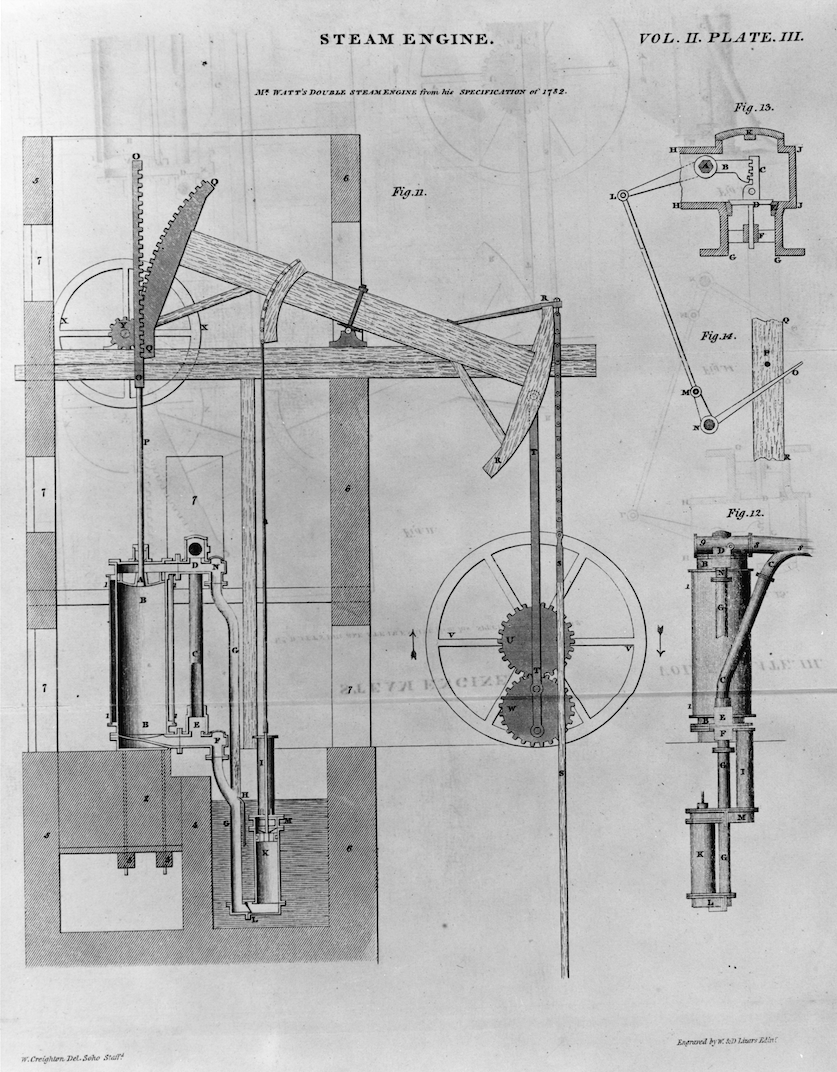
\includegraphics[width=.45\textwidth]{dampfmaschine.png} 
\caption{Dampfmaschine um 1822 \cite{SteamEngin1822}.}
\label{fig:Dampfmaschine}
\end{figure}

\subsubsection{Zweite industrielle Revolution}
Ende des 19. Jahrhunderts wurde damit begonnen, die industrielle Produktion in ihre Teilaufgaben und einzelnen Fertigungsschritte zu zerlegen \parencite{andelfinger2017industrie}. Diese Entwicklung, eng mit den Begriffen \textit{Taylorismus}\footnote{Taylorismus benannt nach dem US-Amerikaner Frederick Winslow Taylor (1856-1915).} und \textit{Fordismus}\footnote{Fordismus benannt nach dem US-amerikanischen Industriellen Henry Ford (1863-1947).} verbunden, erreichte eine weitere Steigerung der Stückzahlen durch die Prozesssteuerung von Arbeitsabläufen.

Der \textit{Taylorismus} verfolgt drei miteinander verbundene Ziele (nach Bonazzi \parencite{bonazzi2014geschichte}):

\begin{itemize}
\item Zentralisierung und Rationalisierung der Weisungsbefugnisse
\item Erhöhung der Produktion und der Leistungsfähigkeit der Arbeiter und der Maschinen durch Reorganisation
\item Nutzung der Wissenschaft zur Betriebsführung durch Normierung von Arbeitsobjekten, Arbeitszeit und Arbeitstätigkeit
\end{itemize}

Während im Taylorismus die Aufmerksamkeit vor allem auf die Organisation der Fabrikarbeit gerichtet wird, konzentriert sich das Konzept des \textit{Fordismus} auf die Größendimension der Produktionseinheiten und die Massenproduktion standardisierter Güter \parencite{bonazzi2014geschichte}. Im Vordergrund steht die Massenproduktion, die durch Starrheit des Produktionsprozesses bzw. durch homogene Produkte charakterisiert wird. 

Auch weniger gut ausgebildete Arbeitskräfte konnten eingesetzt werden, weil jeweils nur ein einzelner Fertigungsschritt der Produktion beherrscht werden mussten. In dieser Zeit entstanden die ersten Fließbandproduktionen (siehe Abb.~\ref{fig:Fliessbandanlage}) und auch die Umstellung auf arbeitsteilige Massenproduktion bzw. Rationalisierung erfolgte \parencite{hocker2015}.

\begin{figure}%[H]
\centering
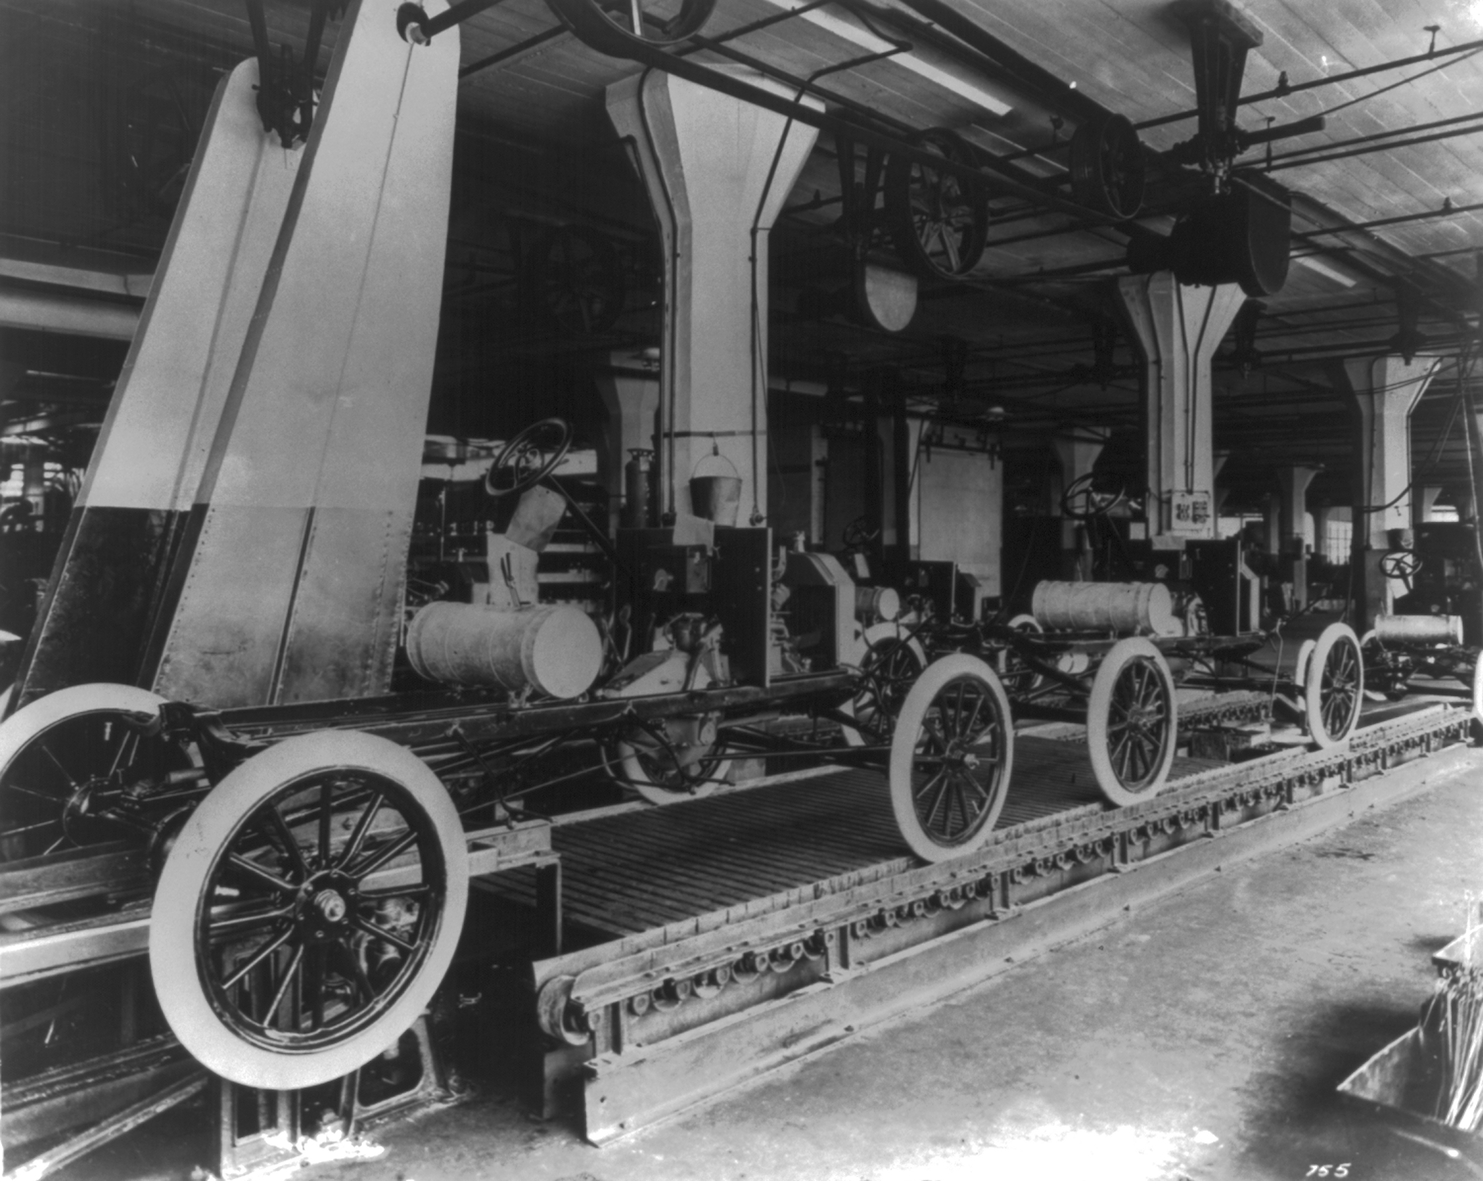
\includegraphics[width=.65\textwidth]{fordFliessband.png} 
\caption{Fließbandanlage Ford Motor Company's Highland Park im Jahr 1913 \cite{FordAssemblyLine1913}.}
\label{fig:Fliessbandanlage}
\end{figure}

\subsubsection{Dritte industrielle Revolution}
Die nächste einschneidende Änderung in der Industrie erfolgte durch den Einsatz von elektronischen Systemen ab Mitte des 20. Jahrhunderts \parencite{andelfinger2017industrie}. Durch den Einsatz von Elektronik und Informationstechnologie (siehe Abb.~\ref{fig:Computeranlage}) waren eine weitere Automatisierung der Produktion und Prozessoptimierungen möglich. Diese Neuerungen führten dazu, dass viele der körperlich schweren oder gefährlichen Arbeiten durch Maschinenanlagen übernommen wurden. Außerdem wurde dadurch eine konstante und höhere Qualität in der Produktion erreicht. Diese Entwicklung wird auch als Informatisierung bzw. Automatisierung bezeichnet \parencite{hocker2015}. 

\begin{figure}%[H]
\centering
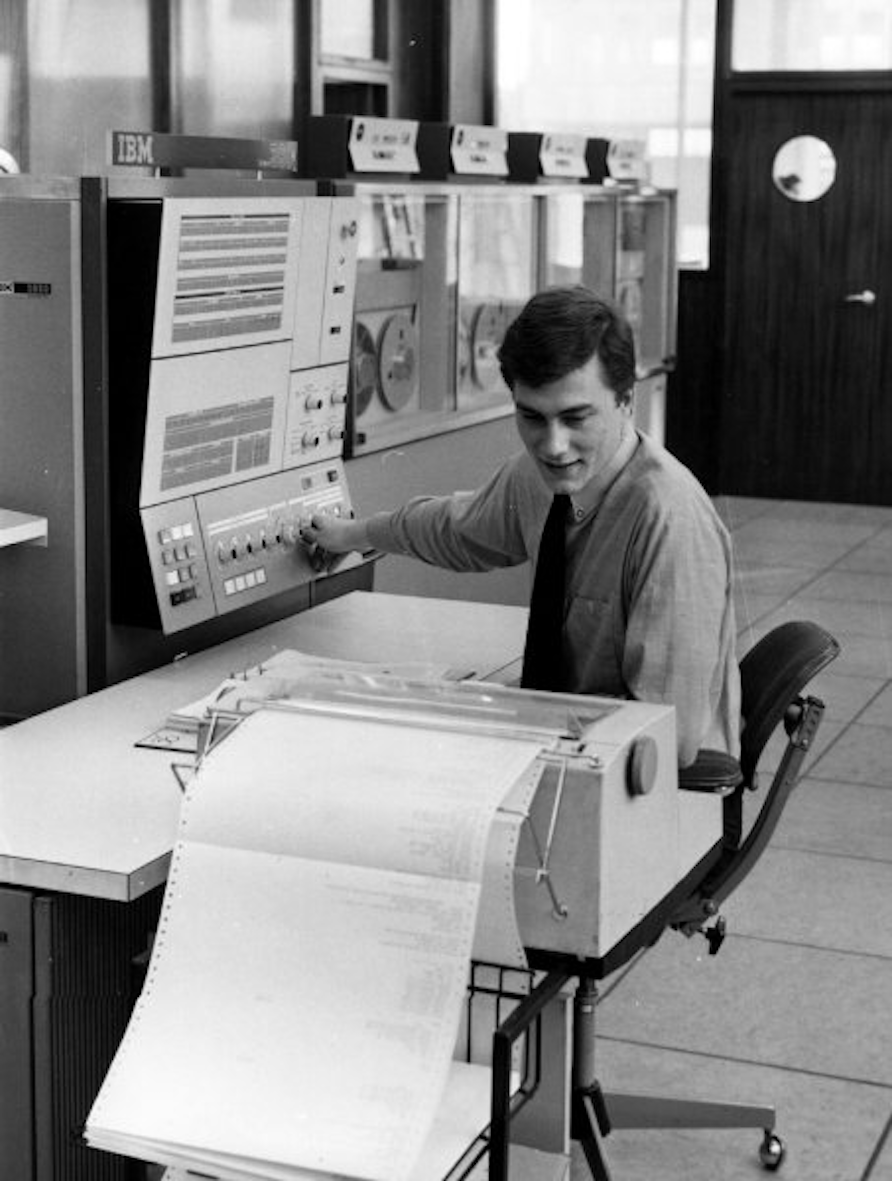
\includegraphics[width=.45\textwidth]{computerRev3.png} 
\caption{Computeranlage aus den 1970er-Jahren \cite{Spiegel}.}
\label{fig:Computeranlage}
\end{figure}

\subsubsection{Industrie 4.0}
Während in der Phase der dritten industriellen Revolution noch jede Betriebsanlage für sich stand und einer zentralisierten Kontrolle unterlag, wird bei der Umsetzung von \textit{Industrie 4.0} der gesamte Lebenszyklus eines Produkts berücksichtigt \parencite{andelfinger2017industrie}. Ein sogenanntes End-To-End-Design wird umgesetzt. Menschen, Dinge und Systeme sind miteinander verbunden und schaffen eine totale Vernetzung. Dadurch entstehen optimierte Wertschöpfungsketten und -netzwerke. 

Ein Integrationskonzept für die Informationsverarbeitung in Produktionsunternehmen vereinigt ein \acl{PPS} mit \acl{CAD} und \acl{CAM}. Cyber-physische Systeme und \acl{M2M}-Kommunikation sind dabei Grundkomponenten. Ein Cyber-physisches System besteht aus mechanischen, elektronischen und softwaretechnischen Komponenten. 

In Abbildung~\ref{fig:AutomotiveShowcase} sieht man eine interaktive Messe- und Ausstellungsapplikation der Firma Siemens Graphscape: "`Siemens Future Forum Industrie 4.0 Automotive Showcase"' als Beispiel, wie eine Produktionsstätte im System Industrie 4.0 organisiert sein kann.

\begin{figure}%[H]
\centering
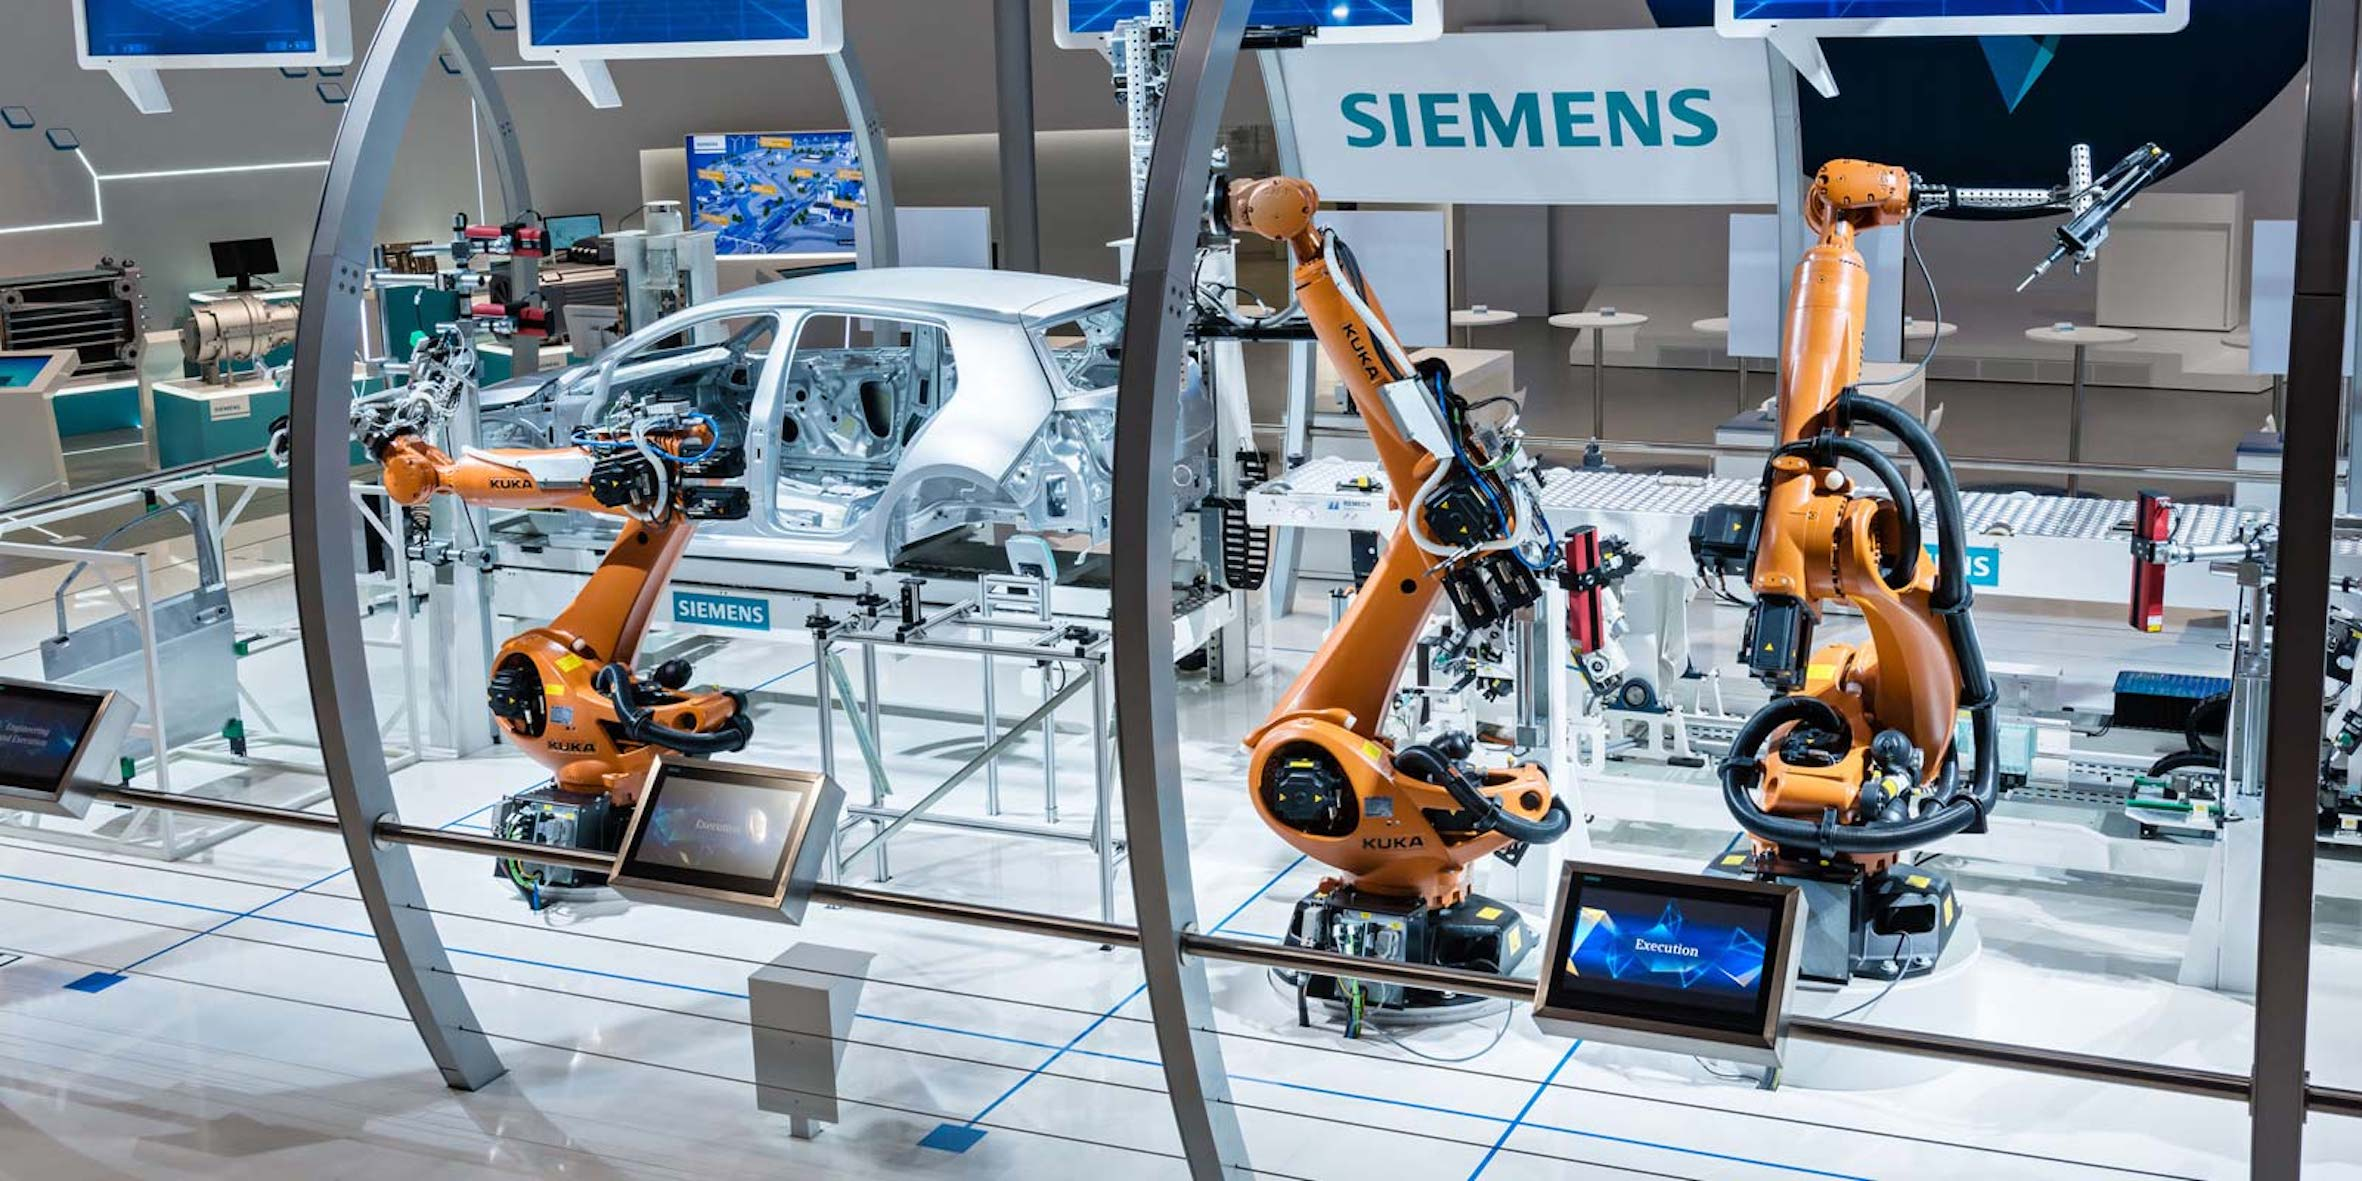
\includegraphics[width=1\textwidth]{siemens_automotive_1.jpg} 
\caption{Siemens Future Forum Industrie 4.0 Automotive Showcase \cite{Siemens}.}
\label{fig:AutomotiveShowcase}
\end{figure}

Industrie 4.0 und \acl{IIoT} sind in den letzten Jahren zu Hauptkonzepten der Industrie geworden und haben weiterhin großes Potential \parencite{gilchrist2016industry}.

\subsection{Hauptcharakteristika und Designprinzipien von Industrie 4.0}
\paragraph{Es gibt folgende vier Hauptcharakteristika von Industrie 4.0 (nach Gilchrist \parencite{gilchrist2016industry}):}
\begin{itemize}
\item vertikale Integration von intelligenten Produktionssystemen:\\
Alle Prozessschritte der Wertschöpfungskette greifen optimal ineinander. Nur so kann auf Ereignisse wie Änderung der Nachfrage oder des Lagerbestands oder  Maschinendefekte rasch reagiert werden. Die vertikale Integration erleichtert auch die kundenspezifische Produktion. 
\item horizontale Integration durch globale Wertschöpfungsnetzwerke:\\
Dies beschreibt das Zusammenspiel der verschiedenen Prozesse der jeweils logischen Ebene -- übergreifend auch auf Partner und Kunden.
\item Einbezug aller Bereiche der Wertschöpfungskette:\\
Der komplette Lebenszyklus eines Produkts von der Herstellung bis zur Entsorgung wird hier betrachtet. Der Fokus liegt dabei auf der Kundenzufriedenheit, erzielt durch Produkte von hoher Qualität.
\item Beschleunigung bzw. Optimierung der Herstellung:\\
Auch bei Industrie 4.0 bleibt dies weiterhin ein unternehmerisches Hauptziel.
\end{itemize}
\vspace{\baselineskip}

\paragraph{Zusätzlich zu den Hauptcharakteristika gibt es noch folgende sechs Designprinzipien für die Umsetzung von Industrie 4.0 (nach Gilchrist \parencite{gilchrist2016industry}):}
\begin{itemize}
\item Interoperabilität zwischen Mensch, intelligenter Fabrik und Technologien:\\
Ein Produktionsprozess verfolgt nicht nur einen gewissen Ablauf, sondern durch Interoperabilität finden ständig Interaktionen zwischen allen Projektpartnern statt. 
\item Virtualisierung (virtueller Zwilling):\\
Eine Virtualisierung der physischen Welt ermöglicht ein einfacheres Modifizieren und Testen des Systems ohne die physischen Prozesse zu beeinträchtigen.
\item Dezentralisierung:\\
Dies erlaubt einzelnen Systemen autonome Entscheidungen innerhalb einer intelligenten Fabrik zu treffen.
\item Echtzeit-Umsetzung:\\
Eine Echtzeit-Umsetzung in Industrie 4.0 umfasst sowohl das Sammeln der Daten als auch das Feedback und das Überwachen der Prozesse.
\item Schwerpunktsetzung auf Service:\\
Interne und externe Services sind in intelligenten Fabriken erforderlich; die Bereitstellung dieser Services wird von Gilchrist als \textit {Schwerpunktsetzung auf Service} bezeichnet \parencite{gilchrist2016industry}.
\item Modularisierung:\\
Um eine möglichst hohe Flexibilität für rasche Anpassung an Veränderungen zu erreichen, sollte bei der Strukturierung auf Modularisierung geachtet werden. Zusätzlich erleichtert dies die Kapselung einzelner Bereiche und die Datenabstraktion.
\end{itemize}
\vspace{\baselineskip}
War es in den 1990er und 2000er-Jahren noch unmöglich, Daten in den erforderlich großen Mengen zu speichern -- weil es einerseits zu teuer und andererseits die Rechenleistung für eine Analyse noch nicht vorhanden war -- ist dies mittlerweile durch Cloud Computing und industrielles Internet möglich. Zusätzlich hat auch die Entwicklung von Smartphones mit Internetzugang rund um 2007 die Entwicklung von Industrie 4.0 weiter vorangetrieben \parencite{gilchrist2016industry}.

\subsection{Ziele von Industrie 4.0}
Ein Ziel von Industrie 4.0 ist es, die Informationstechnik in die Produktion sowie in Produkte und Dienstleistungen zu integrieren \parencite{reinhart2017handbuch}. Dies geschieht durch mehrere Faktoren: 

\begin{itemize}
\item intelligente Fabriken:\\
Im Bereich der Produktion werden intelligente Fabriken entwickelt \parencite{vogel2017handbuch}. Hierbei werden Anlagen mit Sensorik ausgestattet und vernetzt. Durch die intelligente Fabrik sind in der Folge auch intelligente Operationen wie flexible Produktionsplanung und Produktionssteuerung möglich. Zusätzlich gibt es in Industrie 4.0 auch intelligente Produkte, welche auch nach dem Verkauf mit dem Hersteller in Verbindung stehen und datengetriebene Leistungen durch die Vernetzung von Hersteller, Produkt und Kunde bieten.

\item unternehmerische Ziele:\\
Die unternehmerischen Ziele sind hierbei die Effizienzsteigerung durch weitere Automatisierung, kundenindividuelle Produkte zu Kosten eines Massenprodukts, Steigerung des Umsatzes durch digital veredelte Produkte und die Erschließung neuer Märkte \parencite{reinhart2017handbuch}. In einem Industrie 4.0 Unternehmen wird vorausschauend produziert und die Produktion passt sich automatisch an.
\end{itemize}
\vspace{\baselineskip}

Um die Umsetzung von Industrie 4.0 gewinnbringend realisieren zu können, müssen Voraussetzungen in unterschiedlichen Bereichen wie z.B. Organisation, Produktion, Produkte und Services erfüllt werden: 
\begin{itemize}
\item Produktion:\\
In der Produktion muss \ac{IT} eingesetzt werden und eine digitale Repräsentation der Anlagenteile bzw. Assets erfolgen. Die IT-Infrastruktur muss die Daten sammeln und speichern. Danach muss eine Datenanalyse erfolgen, um daraus Erkenntnisse zu gewinnen.

\item Daten:\\
Werden Daten in so großen Mengen gesammelt, dass diese  mit herkömmlichen Datenbanksystemen und Werkzeugen nicht ohne Weiteres verarbeitet werden können, spricht man von \textit{Big Data} \parencite{gilchrist2016industry}. Zusätzlich zur Menge erschwert die große Diversität der Daten die Analyse und auch die Visualisierung. Eine weitere Herausforderung ist es, Daten zu verarbeiten, welche ständig durch neue Einspeisung von Sensordaten vergrößert werden \parencite{stackowiak2015big}. 

\item MitarbeiterInnen:\\
Um den Anforderungen zu entsprechen und die Ziele von Industrie 4.0 zu erreichen müssen die Mitarbeiter eines Unternehmens entsprechend geschult werden und das Informationsmanagement muss im Unternehmen akzeptiert werden.
\end{itemize}
\vspace{\baselineskip} 

Ein Überführen der Produktion in Industrie 4.0 lässt sich in folgende Schritte gliedern (nach Hocker \parencite{hocker2015}):

\begin{itemize}
\item vernetzen und messbar machen (Digitalisierung der Produktion)
\item analysieren und prognostizieren (Spiegelung von physischer in Cyberwelt)
\item Produktion anpassen (simulative Optimierung der Produktion) 
\end{itemize}

\subsection{Standards in Industrie 4.0}
Da es noch keine allgemein gültigen Standards für Industrie 4.0 gibt, haben die Industrieverbände BITKOM\footnote{BITKOM: https://www.bitkom.org} (Bundesverband Informationswirtschaft, Telekommunikation und neue Medien), VDMA\footnote{VDMA: https://www.vdma.org} (Verband Deutscher Maschinen- und Anlagenbau) und ZVEI\footnote{ZVEI: https://www.zvei.org} (Zentralverband Elektrotechnik- und Elektronikindustrie) gemeinsam die Initiative "`Plattform Industrie 4.0"' ins Leben gerufen. Sinn dieser Initiative ist es, Umsetzungsempfehlungen, welche unter anderem die Bereiche Standardisierung, Sicherheit, rechtliche Rahmenbedingungen und Ressourceneffizienz abdecken, festzulegen. 

Auch die Begrifflichkeiten rund um Industrie 4.0 werden je nach Domäne noch sehr unterschiedlich verwendet. Um hier einer Vereinheitlichung näher zu kommen wurde vom Frauenhofer Institut für Optronik, Systemtechnik und Bildauswertung ein Verzeichnis der am häufigsten verwendeten Begriffe erstellt (siehe \parencite{FrauenhoferI40}).

\section{Cloud Computing}
Das \textit{National Institute of Standards and Technology}\footnote{Das \ac{NIST} ist eine Bundesbehörde der USA und hat die Aufgabe, Standards und Richtlinien zu entwickeln. https://www.nist.gov} beschreibt \textit{Cloud Computing} als ein Modell für einen praktischen, On-Demand Netzwerkzugang zu einem IT-In\-fra\-struk\-tur\-sys\-tem. Diese Infrastruktur wird mittels technischer Schnittstellen über den Webbrowser bereit gestellt bzw. abgerufen \parencite{jansen2011sp}.

Amazon war eine der ersten Firmen, die mit \acl{AWS} schon 2006 erste Services in einem Public Cloud System anbot. Weitere Firmen folgten, wie zum Beispiel Microsoft mit Microsoft Azure -- seit 2010 verfügbar -- und Google mit Google Cloud -- seit 2011 verfügbar.

Je nach Art und Umfang der Bereitstellung werden bei Cloud Computing folgende Modelle unterschieden \parencite{jansen2011sp}:

\paragraph{Bereitstellungsmodelle:}
\begin{itemize}
\item Public Cloud:\\ 
Dieses System steht für die breite Öffentlichkeit und unlimitiert vielen Benutzern zur Verfügung.
\item Private Cloud:\\ 
Eine Private Cloud wird exklusiv für eine einzelne Organisation betrieben.
\item Community Cloud:\\ 
Dieses System kann mit einer Private Cloud verglichen werden, jedoch wird eine Community Cloud für zwei oder mehr Kunden betrieben.
\item Hybrid Cloud:\\
Eine Komposition aus mehreren Clouds verschiedener Art wird als Hybrid Cloud bezeichnet.
\end{itemize}

\paragraph{Servicemodelle \parencite{jansen2011sp}:}
\begin{itemize}
\item \ac{SaaS}:\\ 
\ac{SaaS} ist ein Servicemodell, das eine oder mehrere Anwendungen für den Anwender zur Verfügung stellt. Dabei werden für den Kunden die Kosten für Hardware, Softwareentwicklung und Wartung reduziert. Beispiele für \ac{SaaS} sind z.B. Email-Service oder virtueller Desktop.
\item \ac{PaaS}:\\
\ac{PaaS} stellt eine Plattform zur Verfügung, auf welcher vom Kunden Anwendungen entwickelt und bereitgestellt werden können. Im Gegensatz zu \ac{SaaS} hat der Benutzer hier die Kontrolle über Anwendungen und die Entwicklungsumgebung. Beispiele für \ac{PaaS} sind z.B. Execution Runtime, Datenbanken, Web Server und Deployment Tools.
\item \ac{IaaS}:\\
Bei \ac{IaaS} wird von dem Cloud Computing System nur die Grundinfrastruktur zur Verfügung gestellt. Auf dieser Infrastruktur kann der Kunde die gewünschte Entwicklungsplattform aufbauen und seine eigenen Anwendungen entwickeln. Auch die Wahl des Betriebssystems liegt beim Benutzer. Der Konsument ist für die Sicherheit des Systems selbst verantwortlich. Beispiele für \ac{IaaS} sind Speicherplatz und virtuelle Maschinen.
\end{itemize}
\vspace{\baselineskip}

Abbildung~\ref{fig:cloud} zeigt die Unterschiede von Zugriff und Kontrolle der verschiedenen Cloud Service Modelle -- bei \ac{SaaS} liegt die Verantwortung ausschließlich beim Cloud Betreiber während bei \ac{IaaS} ein großer Teil beim Cloud Nutzer liegt.

\begin{figure}%[!h]
\centering
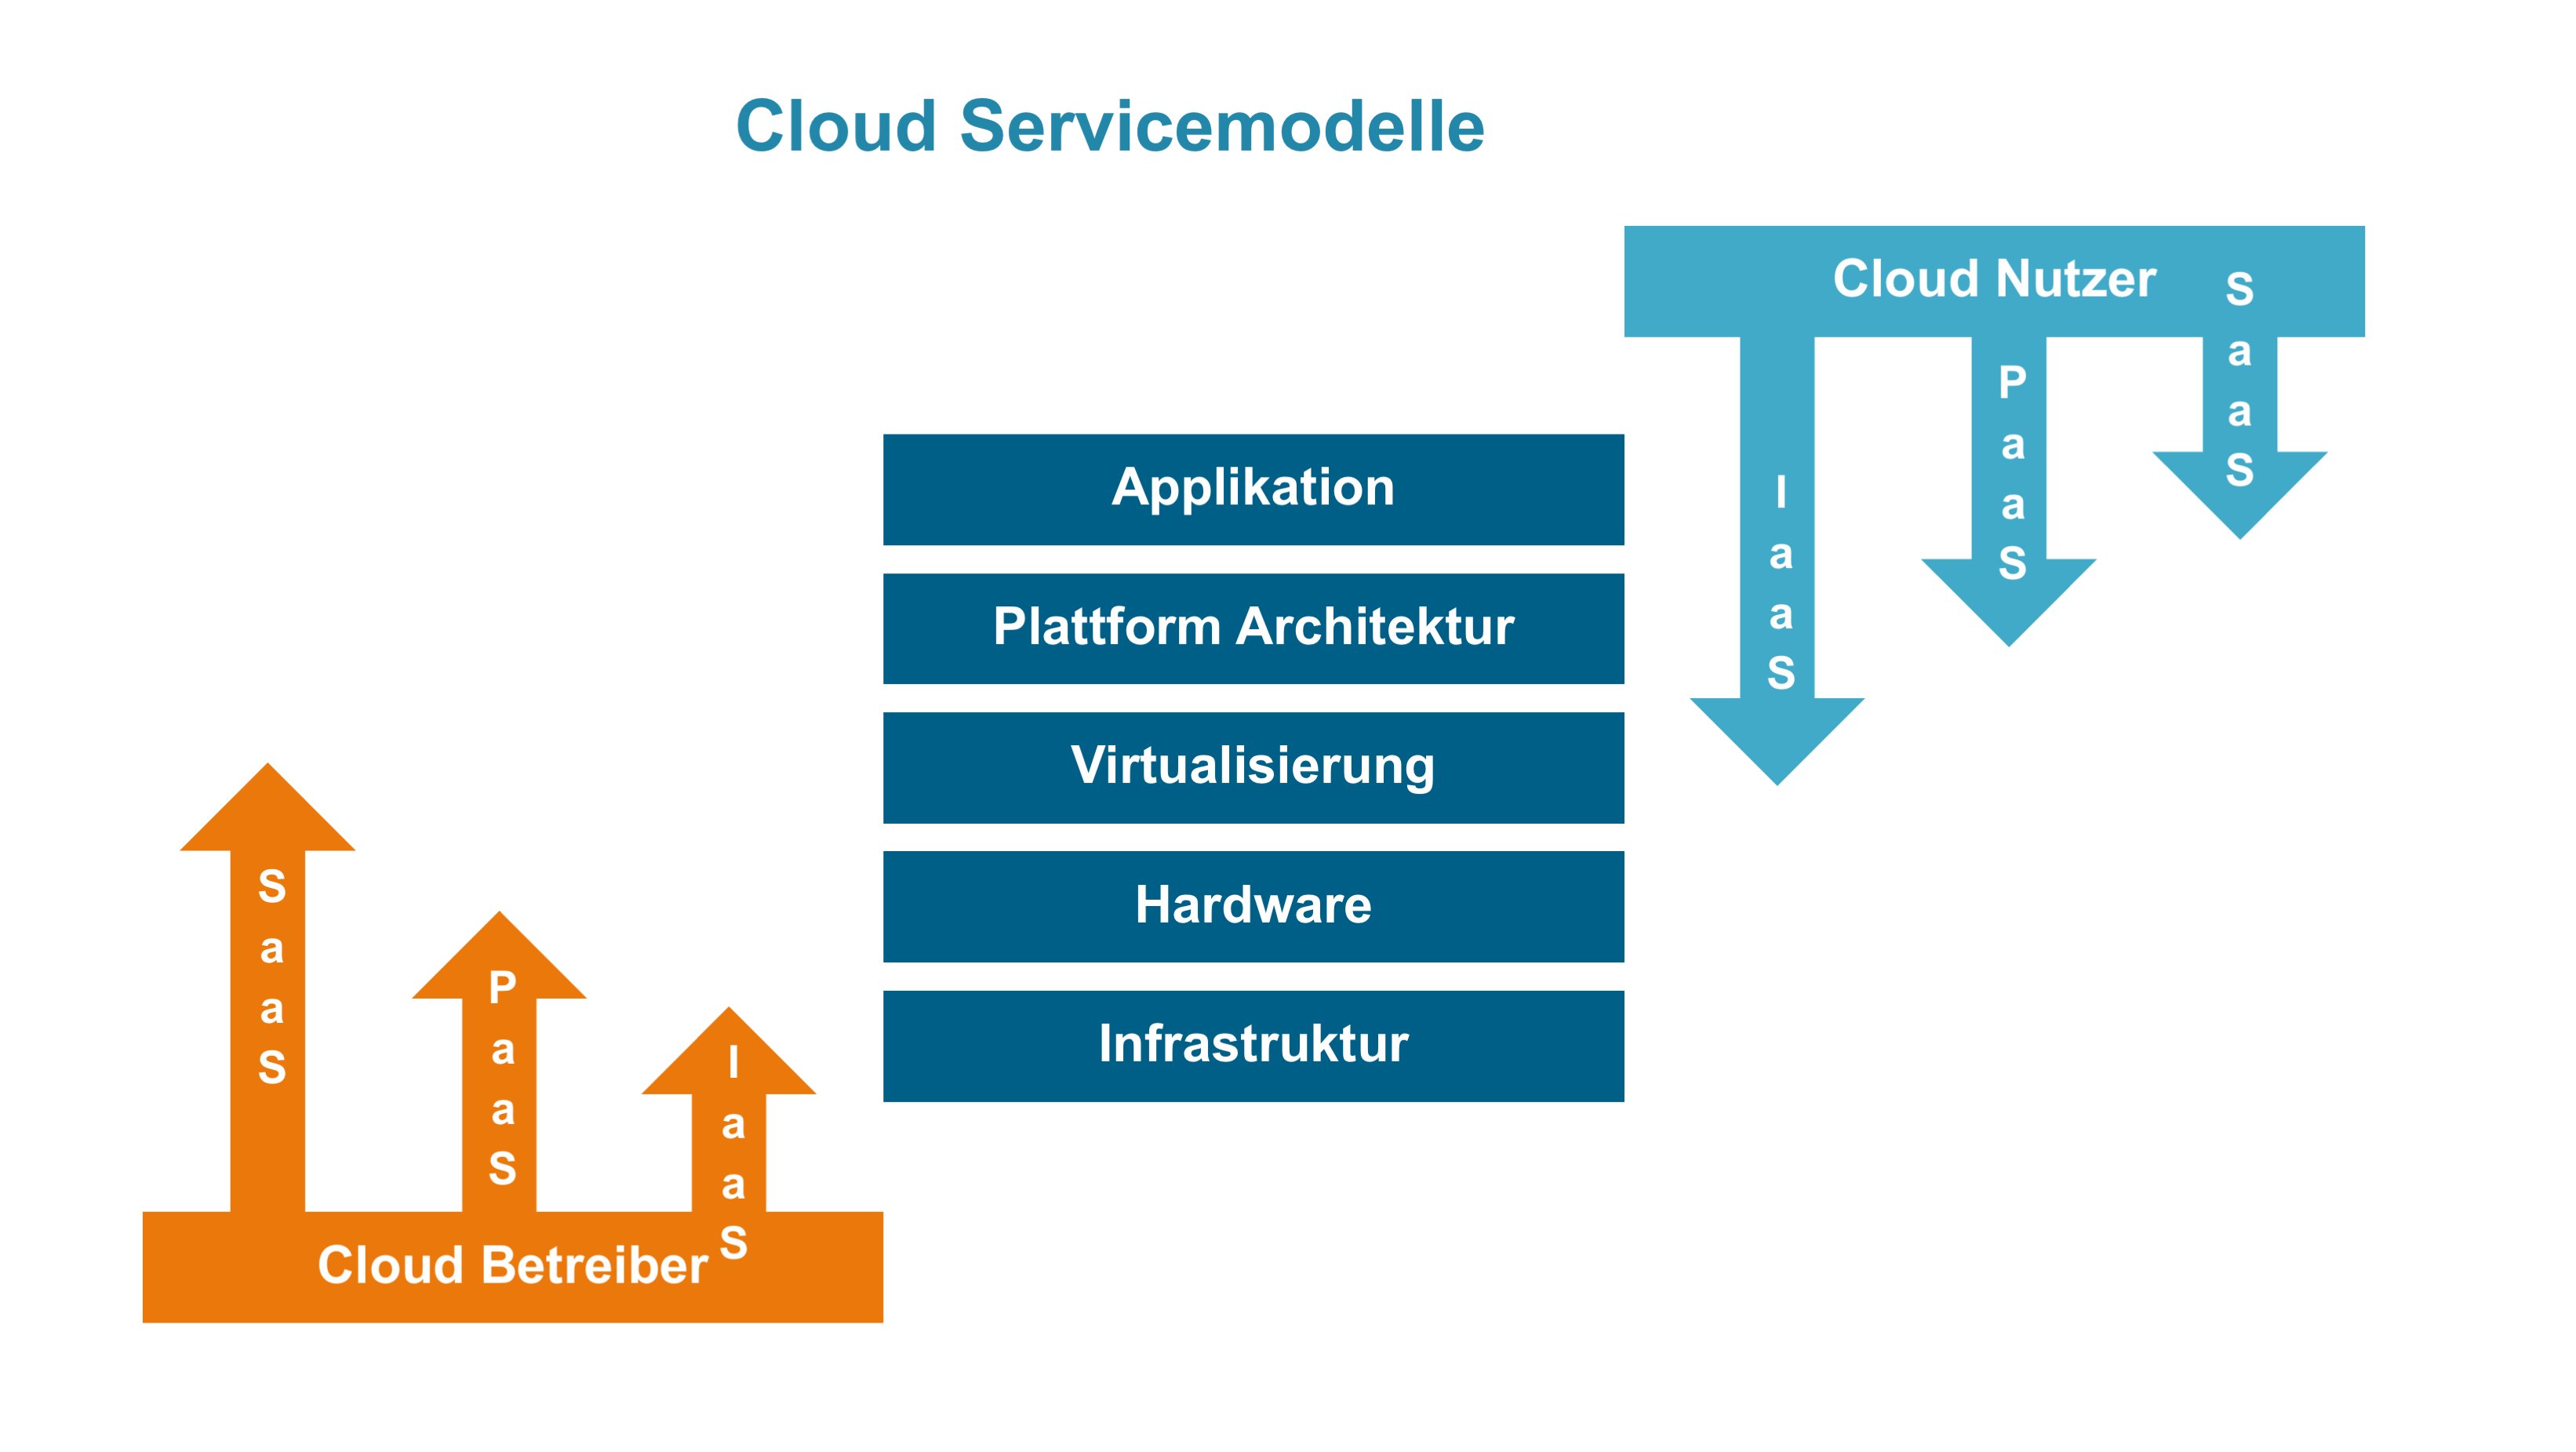
\includegraphics[width=1\textwidth]{CloudServiceModelle.png} 
\caption{Unterschiede in Zugriff und Kontrolle bei Cloud Servicemodellen (vgl. \cite{gilchrist2016industry}).}
\label{fig:cloud}
\end{figure}

\section{Begriffsabgrenzung "`Internet of Things"'}
Im Bereich von \textit{\ac{IoT}} oder Internet der Dinge werden die Begriffe \ac{IoT}, \acl{IoE}, \acl{IIoT} und Internet 4.0 beinahe gleichbedeutend verwendet \parencite{gilchrist2016industry, stackowiak2015big}. Während General Electric den Terminus "`Industrielles Internet"' prägte, entstand im Umfeld von Cisco der Begriff "`\ac{IoE}"'. Der US-amerikanische Wissenschafter Kevin Ashton verwendete 1999 zum ersten Mal den Begriff \ac{IoT} \parencite{ashton2011internet}. 

\subsection{Internet of Things}
\ac{IoT} bezeichnet jene allgegenwärtigen Dinge oder Objekte (z.B. \acl{RFID} Tags, Sensoren), welche mit ihren Nachbarn interagieren, kommunizieren und kooperieren, um gemeinsame Ziele zu erreichen \parencite{batallabeyond}. Die Kommunikation erfolgt dabei mit Hilfe des Internets. Zusätzlich werden diese Vorgänge mit einem Minimum an menschlicher Intervention durchgeführt. Die Trennung zwischen physischer und virtueller Welt verschwindet dabei \parencite{vogel2017handbuch}. 

\ac{IoT} besteht aus physischen Objekten unterschiedlichster Art (z.B. Anlagen, Maschinen oder Sensoren). Dabei benötigen alle Teilnehmer eine eindeutige Identifizierung.  

Bereits in den 1970er-Jahren gab es erste Versuche, ein Netzwerk innerhalb von "`Dingen"' aufzubauen \parencite{jeschke2017industrial}. Ein Sammelbegriff dafür ist \ac{CIM}. Diese Technologie stieß jedoch noch auf Grenzen. Diese lagen darin, dass die \acl{IKT} noch unausgereift war, Computer eine noch zu geringe Rechenleistung hatten und zu kleine Datenspeicher zur Verfügung standen. Darüber hinaus waren die Übertragungsraten zu klein und Software Tools und Formate für den Datenaustausch fehlten.

Mittlerweile haben sich die technischen Möglichkeiten in vielen Bereichen stark verbessert. Zum Beispiel haben sich in der Sensortechnologie die Größe und die Kosten der einzelnen Sensoren in den letzten Jahren massiv reduziert sowie die Verlässlichkeit verbessert, sodass immer mehr Betriebe auf diese Technologie vertrauen. Das Miniaturisieren der Sensoren ist soweit vorangeschritten, dass es aktuell Sensoren mit der Größe von Sandkörnern gibt \parencite{gilchrist2016industry}.

Von Siemens AG, Digital Factory, wurden 2017 folgende Zahlen bzgl. Siemensprodukte bekannt gegeben: 30 Millionen Automatisierungssysteme, 70 Millionen Smart Meters und 800.000 verbundene Produkte sind derzeit aktiv.

Laut einer Studie der Siemens AG werden derzeit rund 5,5 Millionen "`Dinge"' pro Tag neu vernetzt. Eine Prognose von Siemens AG schätzt, dass sich die Anzahl der verbundenen Assets im Zeitraum von 2017 bis 2020 annähernd verdoppeln  und ca. 50 Milliarden umfassen wird (siehe Abb.~\ref{fig:NumberOfAssets}).

\begin{figure}%[H]
\centering
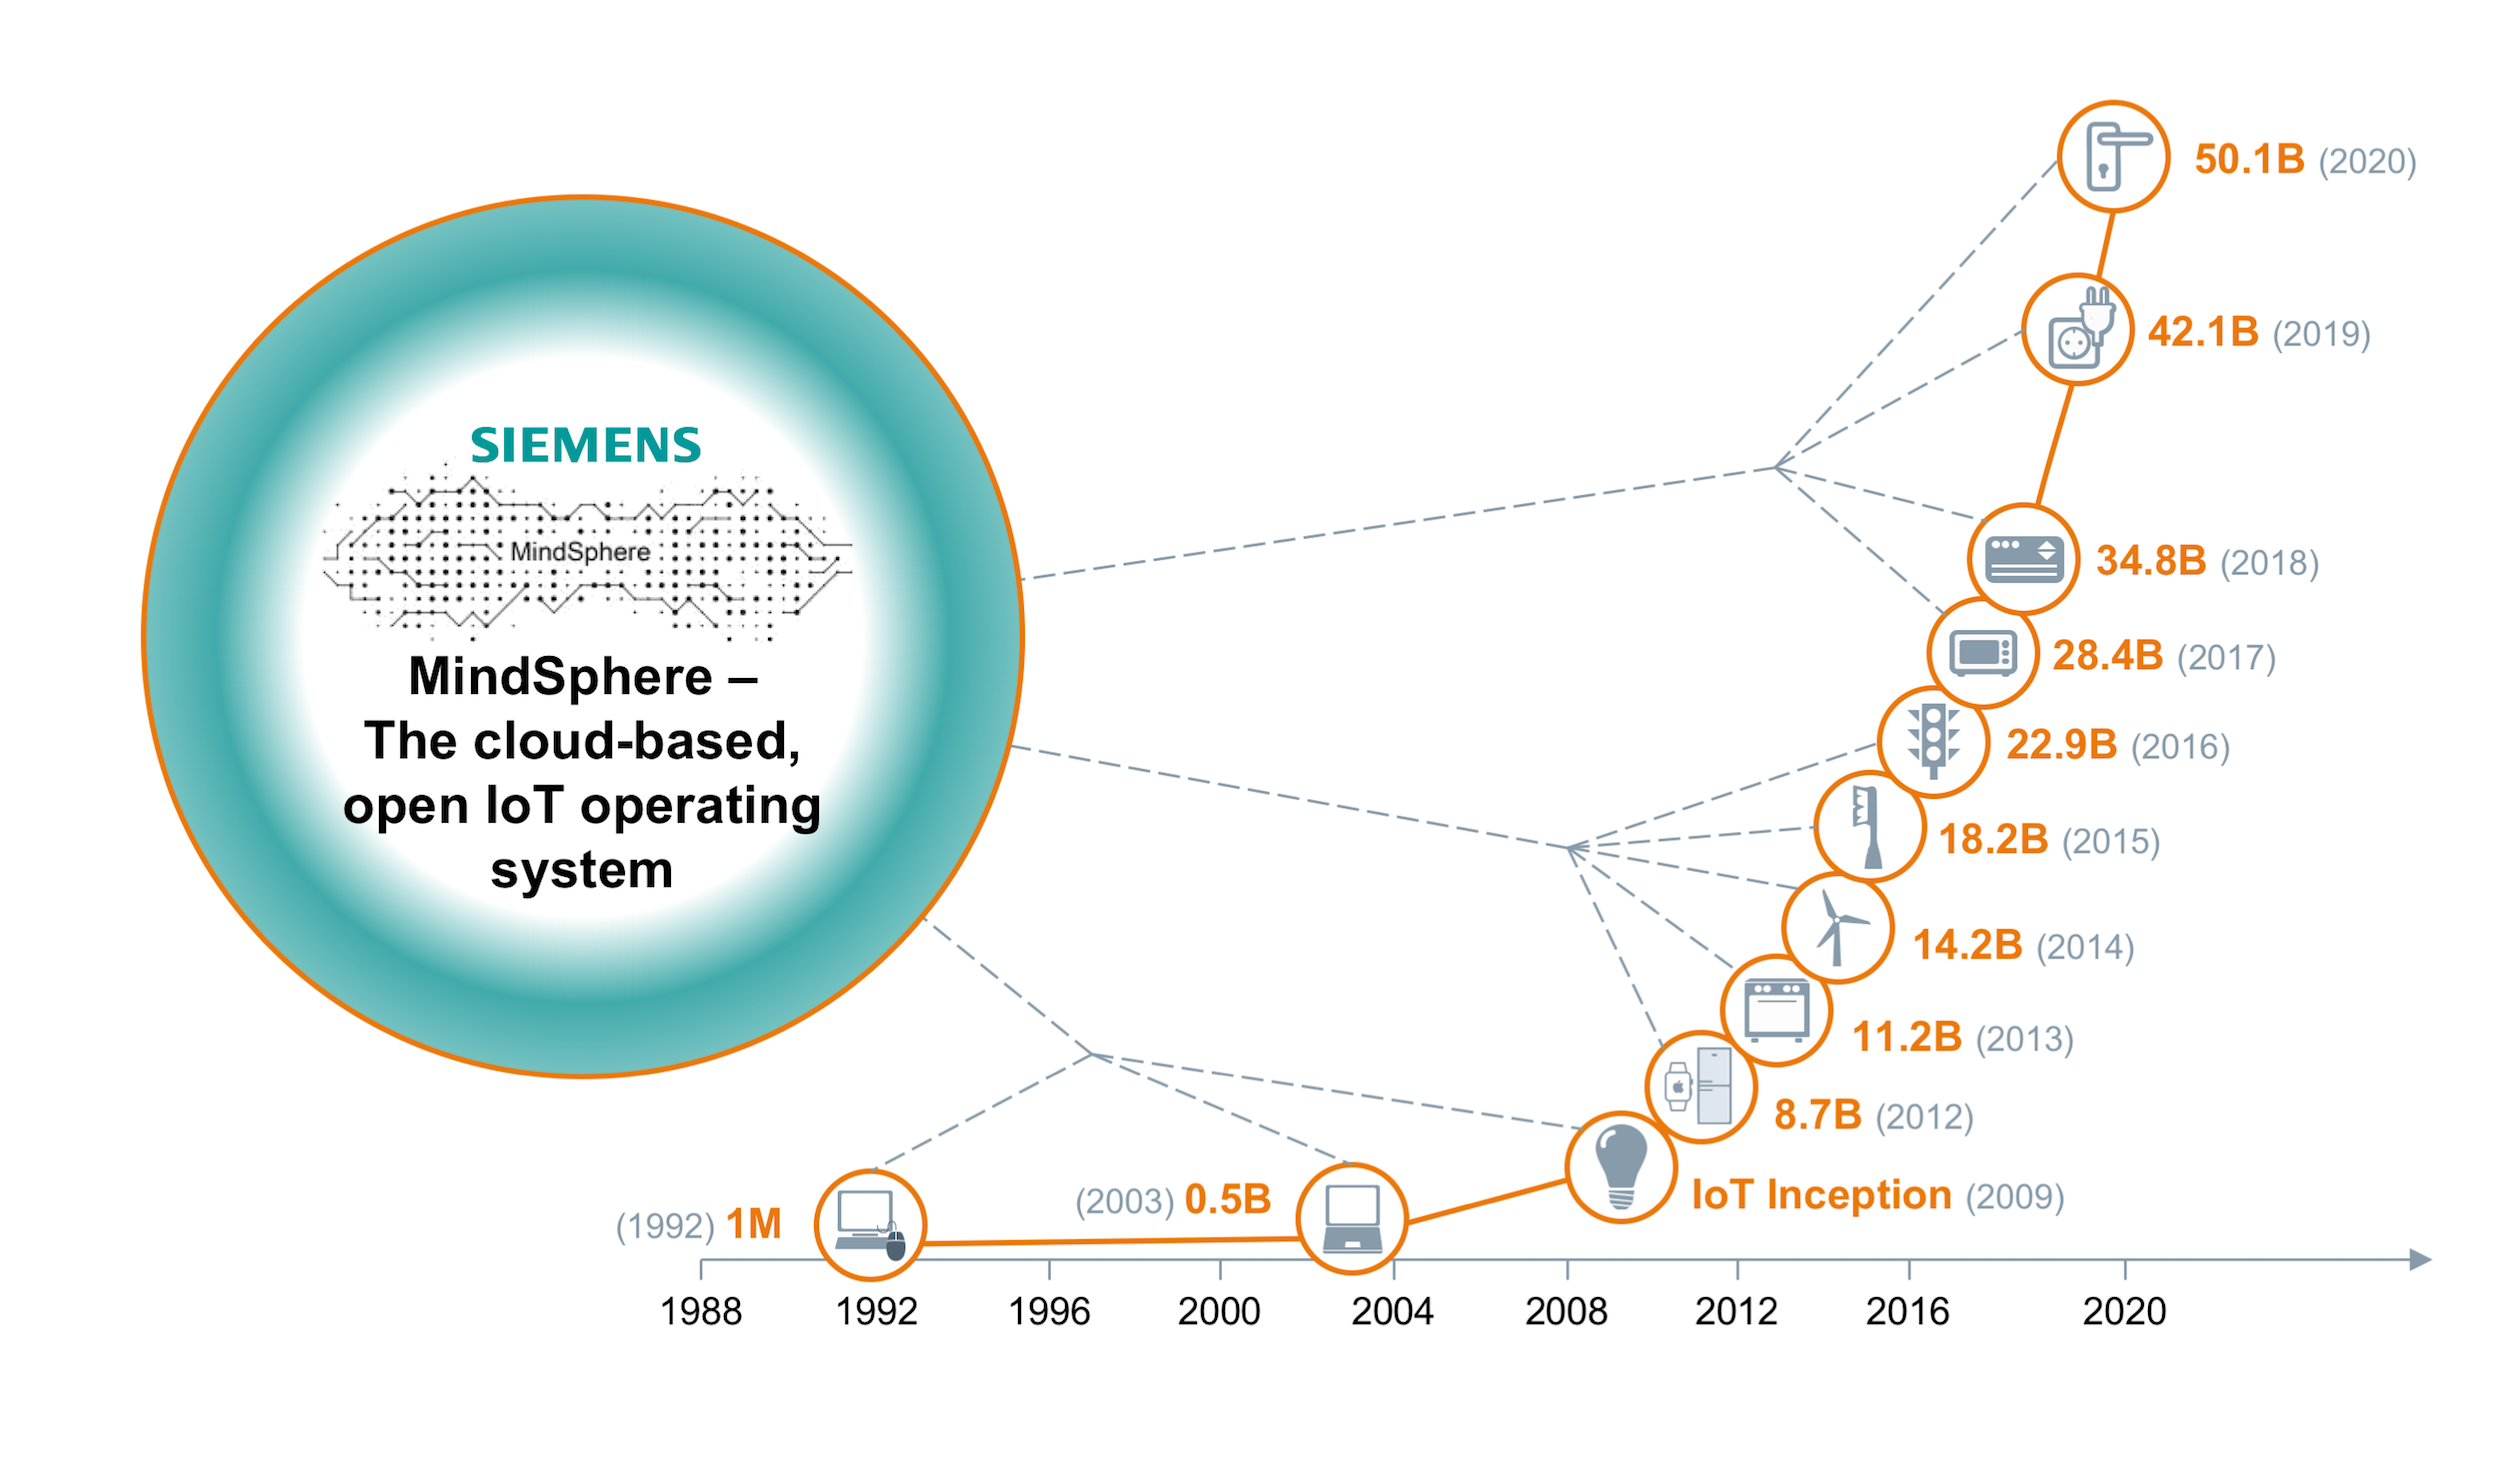
\includegraphics[width=1\textwidth]{NumberOfAssets_2.png} 
\caption{Darstellung des prognostizierten Anstiegs der Anzahl der verbundenen Assets \cite{SiemensMSIntroduction}.}
\label{fig:NumberOfAssets}
\end{figure}

\subsection{Internet of Everything}
Im Unterschied zu \ac{IoT} beschränkt sich \ac{IoE} nicht nur auf die Dinge, welche über das Internet verbunden werden, sondern bezieht auch den Menschen direkt mit ein. Die Interaktion Mensch-Gerät soll dadurch vereinfacht und erleichtert werden \parencite{andelfinger2014internet}. 

\ac{IoE} kann also auch als Netzwerk, welches Menschen, Dinge, Prozesse und Daten verbindet, bezeichnet werden; Verbindungen werden automatisiert und Menschen selbst zu "`Internetknoten"' \parencite{batallabeyond}. Ziel ist es, schnelle persönliche Kommunikation zu ermöglichen und neue Information sichtbar zu machen.

Bisher verbinden sich Menschen aktiv mit Hilfe verschiedener Geräte mit dem Internet. Durch \ac{IoE} verbinden sich unterschiedlichste Geräte im Umkreis von Personen selbständig mit dem Internet \parencite{batallabeyond}.
 
"`Wearables"' stellen einen speziellen Bereich von \ac{IoE} dar. Dabei handelt es sich um Gegenstände, welche mit Sensoren ausgestattet sind und am oder im Körper getragen werden \parencite{andelfinger2014internet}. Dabei kann es sich zum Beispiel um intelligente Ringe oder andere Schmuckstücke handeln, welche permanent den Blutdruck oder andere Vitalfunktionen ihres Trägers messen. 

Ein weiterer Einsatz von Wearables im medizinischen Bereich sind zum Beispiel Tabletten mit integrierten Sensoren \parencite{batallabeyond}. Falls es sich dabei um lebenserhaltende Medikamente handelt, wird über die Sensoren festgestellt, ob die Einnahme zeitgerecht erfolgt ist. Ist die Einnahme nicht erfolgt, wird eine automatische Alarmierung und in Folge eine Rettungskette direkt über die Datenübertragung der Sensoren eingeleitet \parencite{batallabeyond}. Ansonsten senden die Sensoren diverse Messdaten direkt vom Verdauungstrakt an den behandelten Arzt.

Weitere Beispiele für \ac{IoE} findet man in den Bereichen Smart Home und Home Automation, Smart Grid und \acl{AR}.

\subsection{Industrial Internet of Things}
Im industriellen Umfeld wird die Anwendung von \acl{IoT} oft als \ac{IIoT} bezeichnet, welches Thema des 46. World Economic Forum 2016 in Davos war.

Industrielles Internet steht noch immer am Beginn seiner Entwicklung. Sensoren und Geräte (Devices), welche Daten zur Kontrolle von Operationen liefern, gibt es schon seit vielen Jahren. Außerdem gibt es schon lange \ac{M2M} Kommunikation. Also ist der Kern von \ac{IIoT} eigentlich nichts Neues \parencite{gilchrist2016industry}. Wie in Abbildung~\ref{fig:M2MIIoT} erkennbar, unterscheiden sich die Architekturen von \ac{M2M} und \ac{IIoT} lediglich durch das Einbinden der Cloud-Komponente \parencite{gilchrist2016industry}.

\begin{figure}%[H]
\centering
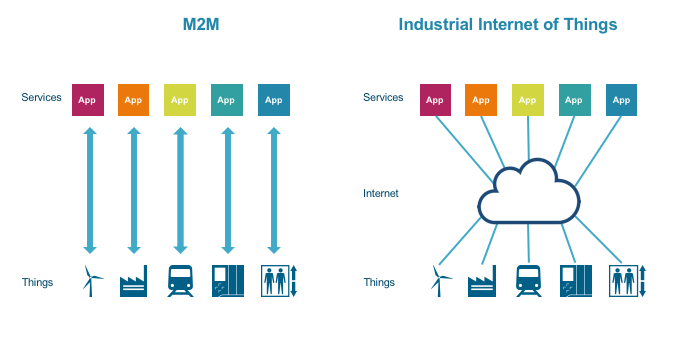
\includegraphics[width=1\textwidth]{M2M_IIoT.png} 
\caption{Gegenüberstellung Architekturen \ac{M2M} und \ac{IIoT} (vgl.\cite{gilchrist2016industry}).}
\label{fig:M2MIIoT}
\end{figure}

Der Hauptnutzen von \ac{IIoT} ist eine bessere Sichtbarkeit und mehr Einblick in die Operationen eines Betriebes \parencite{gilchrist2016industry}. Weitere Ziele liegen darin, erhöhte Profite zu erzielen, schnellere und optimierte Prozesse zu erhalten, die Ausgaben zu reduzieren und die Gesundheit und Sicherheit der Mitarbeiter in der Produktion zu steigern. 

Gegenüber einfacher \ac{M2M} Kommunikation ist die Skalierung von \ac{IIoT} eine andere: Daten können hier mit Hilfe von IIoT-Systemen in Cloud Systemen gesammelt, gespeichert, analysiert und zurück zum Gerät als Kontroll-Feedback geschickt werden. 

Dabei wird die gesamte Produktionskette vernetzt; Maschinen können miteinander kommunizieren und einzelne Produktionsschritte selbstständig steuern \parencite{andelfinger2014internet, gilchrist2016industry}. Voraussetzung dafür ist, dass sämtliche Maschinen bzw. Anlagenteile mit Sensoren ausgestattet werden. In der Folge werden präzise Daten zum Status der Maschinen sowie zu den erzeugten Produkten geliefert. Optimierungen der Produktionsabläufe sowie eine möglichst einfache und kostenschonende Wartung sind dabei das Ziel. Erst dadurch wird eine vorausschauende Arbeit und teilweise auch Selbstdiagnose der Maschinen möglich.

Die Steuerung der Produktionsprozesse in intelligenten Fabriken (Smart Factories) oder auch digitalen Fabriken (Digital Factories) (siehe Abb.~\ref{fig:smartFactory}) erfolgt automatisiert und Eingriffe von außen werden minimiert.

\begin{figure}%[H]
\centering
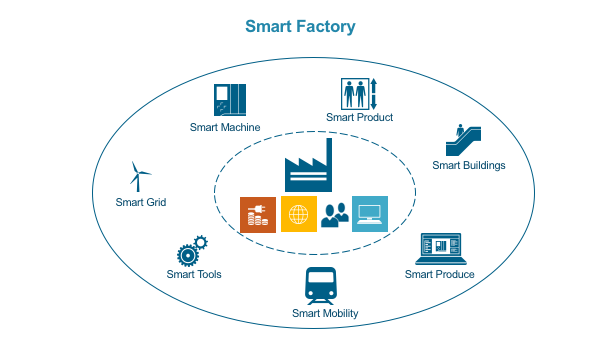
\includegraphics[width=1\textwidth]{SmartFactory.png} 
\caption{Struktur Smart Factory (vgl.\cite{gilchrist2016industry}).}
\label{fig:smartFactory}
\end{figure}

Die Vernetzung der Maschinen geht über einzelne Fabriken hinaus und vernetzt ebenso Partnerfabriken und Lieferanten bis hin zum Kunden \parencite{andelfinger2014internet}. Die Rolle des Menschen reduziert sich hier auf die Überwachung und die Entwicklung von Produktionsprozessen.

\paragraph{Einige Anwendungsgebiete von industriellem Internet (nach Gilchrist \parencite{gilchrist2016industry}):}
\begin{itemize}
\item Logistik
\item Transport
\item Luftfahrt
\item Gesundheit
\item Energieproduktion
\item Öl- und Gasförderung
\item Smart Office
\item Smart Homes - Gebäudeautomation
\end{itemize}
\vspace{\baselineskip}


\section{Siemens MindSphere}
Die Firma Siemens AG bietet seit Juli 2016 mit MindSphere\footnote{MindSphere: https://www.siemens.com/global/de/home/produkte/software/mindsphere.html} ein cloud-basiertes, offenes \ac{IoT}-Betriebssystem auf der Basis von \ac{PaaS} für digitale Services an \parencite{SiemensMSIntroduction,SiemensWhitepaper}. Industrielle Anlagen können so auf einfache Weise Daten in eine Cloud-Umgebung liefern und auch wieder abgreifen. 

\subsection{Motivation für MindSphere}

Daten von zahlreichen, bereits installierten Geräten und Maschinen werden gesammelt und in definierten Intervallen in eine Cloud übertragen. Von dort können diese Daten jederzeit wieder abgerufen bzw. ausgewertet werden. Hauptmotivation ist die Performance bzw. Leistung von sogenannten Assets\footnote{Asset bedeutet im Umfeld von MindSphere eine digitale und logische Repräsentation einer physischen Maschine oder eines Anlagenteils.} zu steigern. Mehrere ähnliche oder sogar gleiche Anlagen oder Arbeitsabläufe können somit direkt verglichen und in der Folge sowohl in Bezug auf Kosten als auch auf Herstellungszeit des Produkts optimiert werden.

Ein weiterer Aspekt ist die vorausschauende und vorbeugende Wartung -- \ac{PPM}.  Unter \ac{PPM} versteht man, dass auf Grund von stark abweichenden Daten ein Ausfall eines Anlagenteils möglichst früh und mit hoher Wahrscheinlichkeit vorausgesagt werden kann und dadurch der Wartungsaufwand und die eventuelle Ausfallszeit einer Anlage minimiert werden können. 

Mit der Datenanalyse kann auch eine Qualitätsanalyse und in der Folge eine Qualitätssteigerung der Produkte durchgeführt werden. Auch für das Garantiemanagement sind die Daten von großem Nutzen. 

Zusammenfassend sind die Ziele eine Senkung der Produktions- und Wartungskosten sowie eine Steigerung der Anlagenleistung und User Experience. Als User Experience werden die Wahrnehmungen und Reaktionen einer Person aufgrund der Nutzung eines Produkts, eines Systems oder einer Dienstleistung bezeichnet \parencite{dis20099241, hartson2012ux}.

\subsection{Aufbau MindSphere }
MindSphere ist aus drei Schichten aufgebaut (siehe Abb.~\ref{fig:MSArchitecture}) \parencite{SiemensMSIntroduction,SiemensWhitepaper}. In der untersten Schicht (Ebene 1 -- Konnektivität) erfolgt der direkte Zugang zu den physischen Geräten, in der mittleren Schicht (Ebene 2 -- Plattform) befindet sich die Cloud-Infrastruktur und in der obersten Schicht (Ebene 3 -- Applikationen) befinden sich die Applikationen.

\begin{figure}[H]
\centering
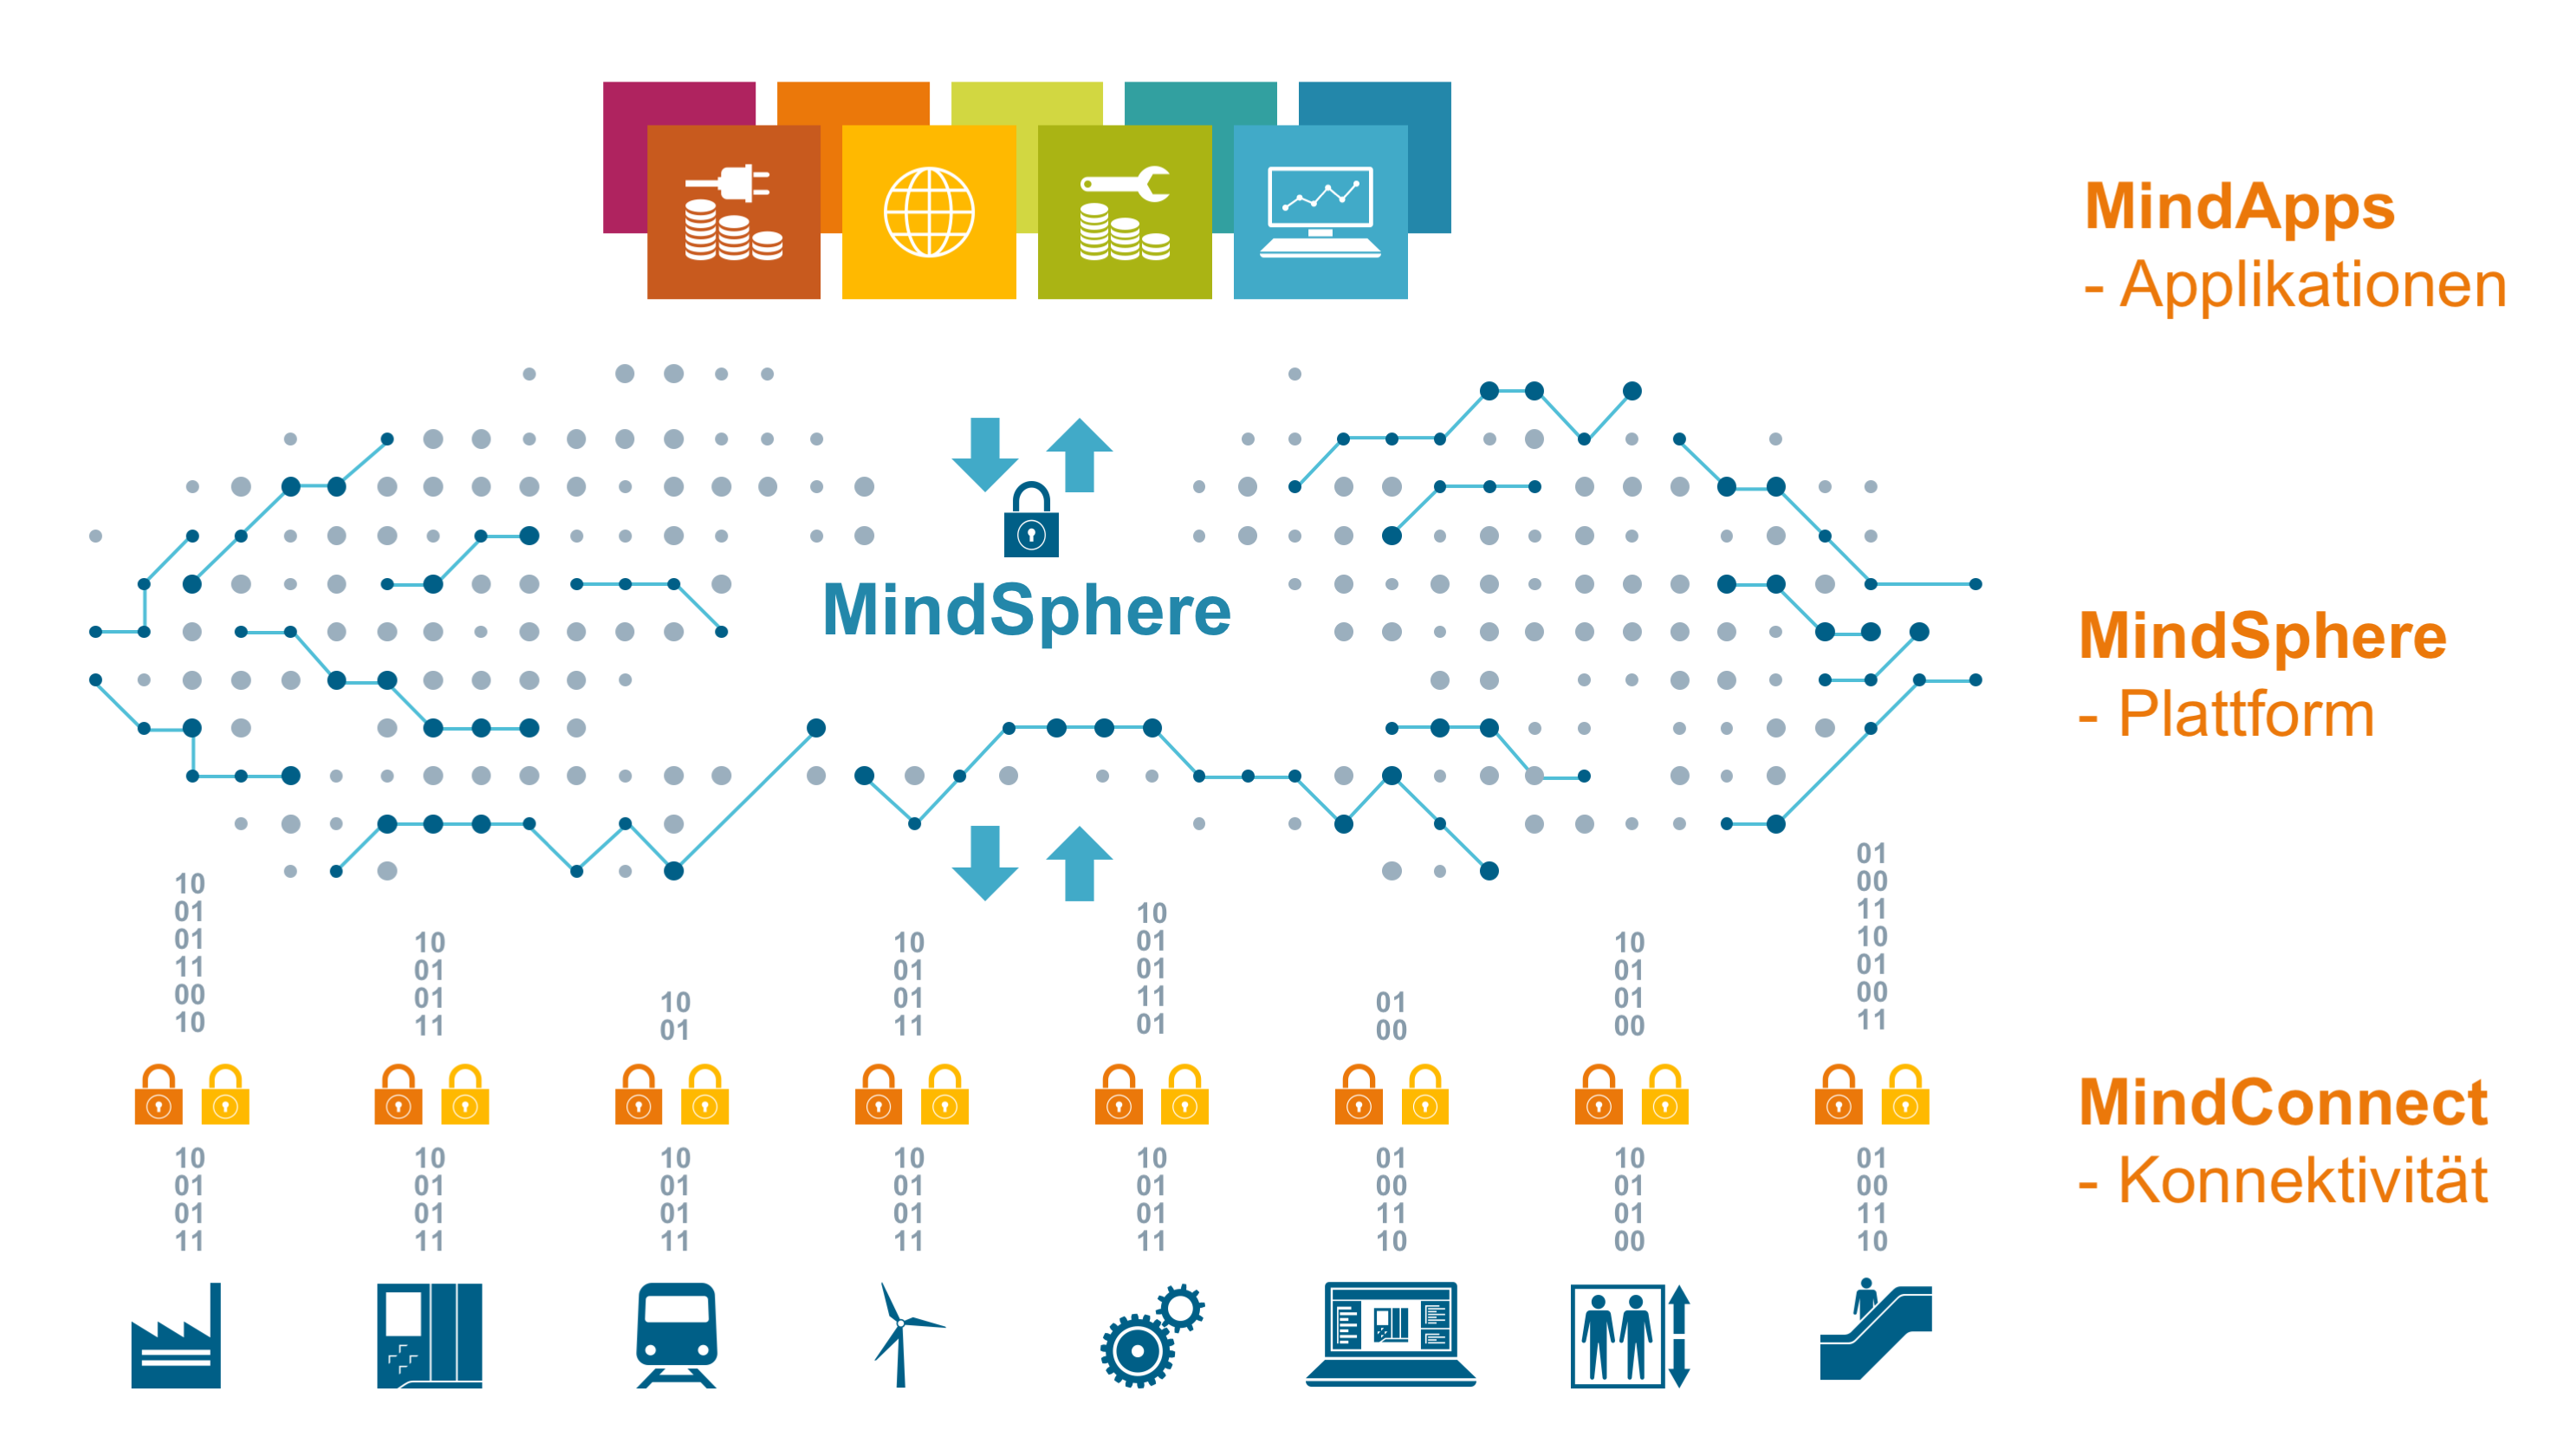
\includegraphics[width=1\textwidth]{MSArchitektur_1.png} 
\caption{Aufbau von MindSphere in drei Ebenen \cite{SiemensMSIntroduction}.}
\label{fig:MSArchitecture}
\end{figure}

\subsubsection{MindConnect}
Auf Ebene 1 -- Konnektivität -- wird durch \textit{MindConnect} eine Schnittstelle zwischen einer speicherprogrammierbaren Steuerung (\acs{SPS}) und der MindSphere Cloud hergestellt. 

Die Kommunikation zwischen den Assets und den MindConnect-Modulen erfolgt derzeit\footnote{Stand November 2017} mittels Open Standard Kommunikation wie z.B. OPC UA (Open Platform Communications Unified Architecture) oder Siemens S7 300/400 Protokoll. Für die nächste Version ist auch eine Unterstützung von z.B. MODBUS geplant. 

MindConnect bezeichnet ein physisches Gerät, welches vor Ort direkt in der Betriebsanlage an die \acs{SPS} montiert und durch Plug-and-Play verbunden wird. Hier bietet die Firma Siemens zwei Hardware-Komponenten an (siehe Abb.~\ref{fig:MSConnect}):
\vspace{\baselineskip}

\begin{figure}[H]
\centering\small
\setlength{\tabcolsep}{0mm}
\begin{tabular}{c@{\hspace{12mm}}c}
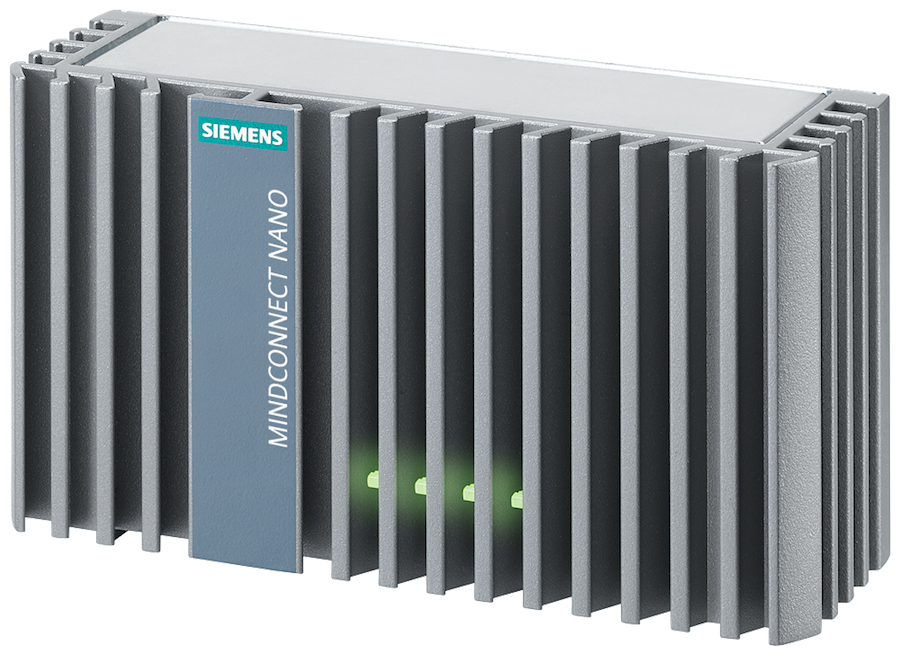
\includegraphics[width=0.45\textwidth]{MindConnect_Nano.png}&
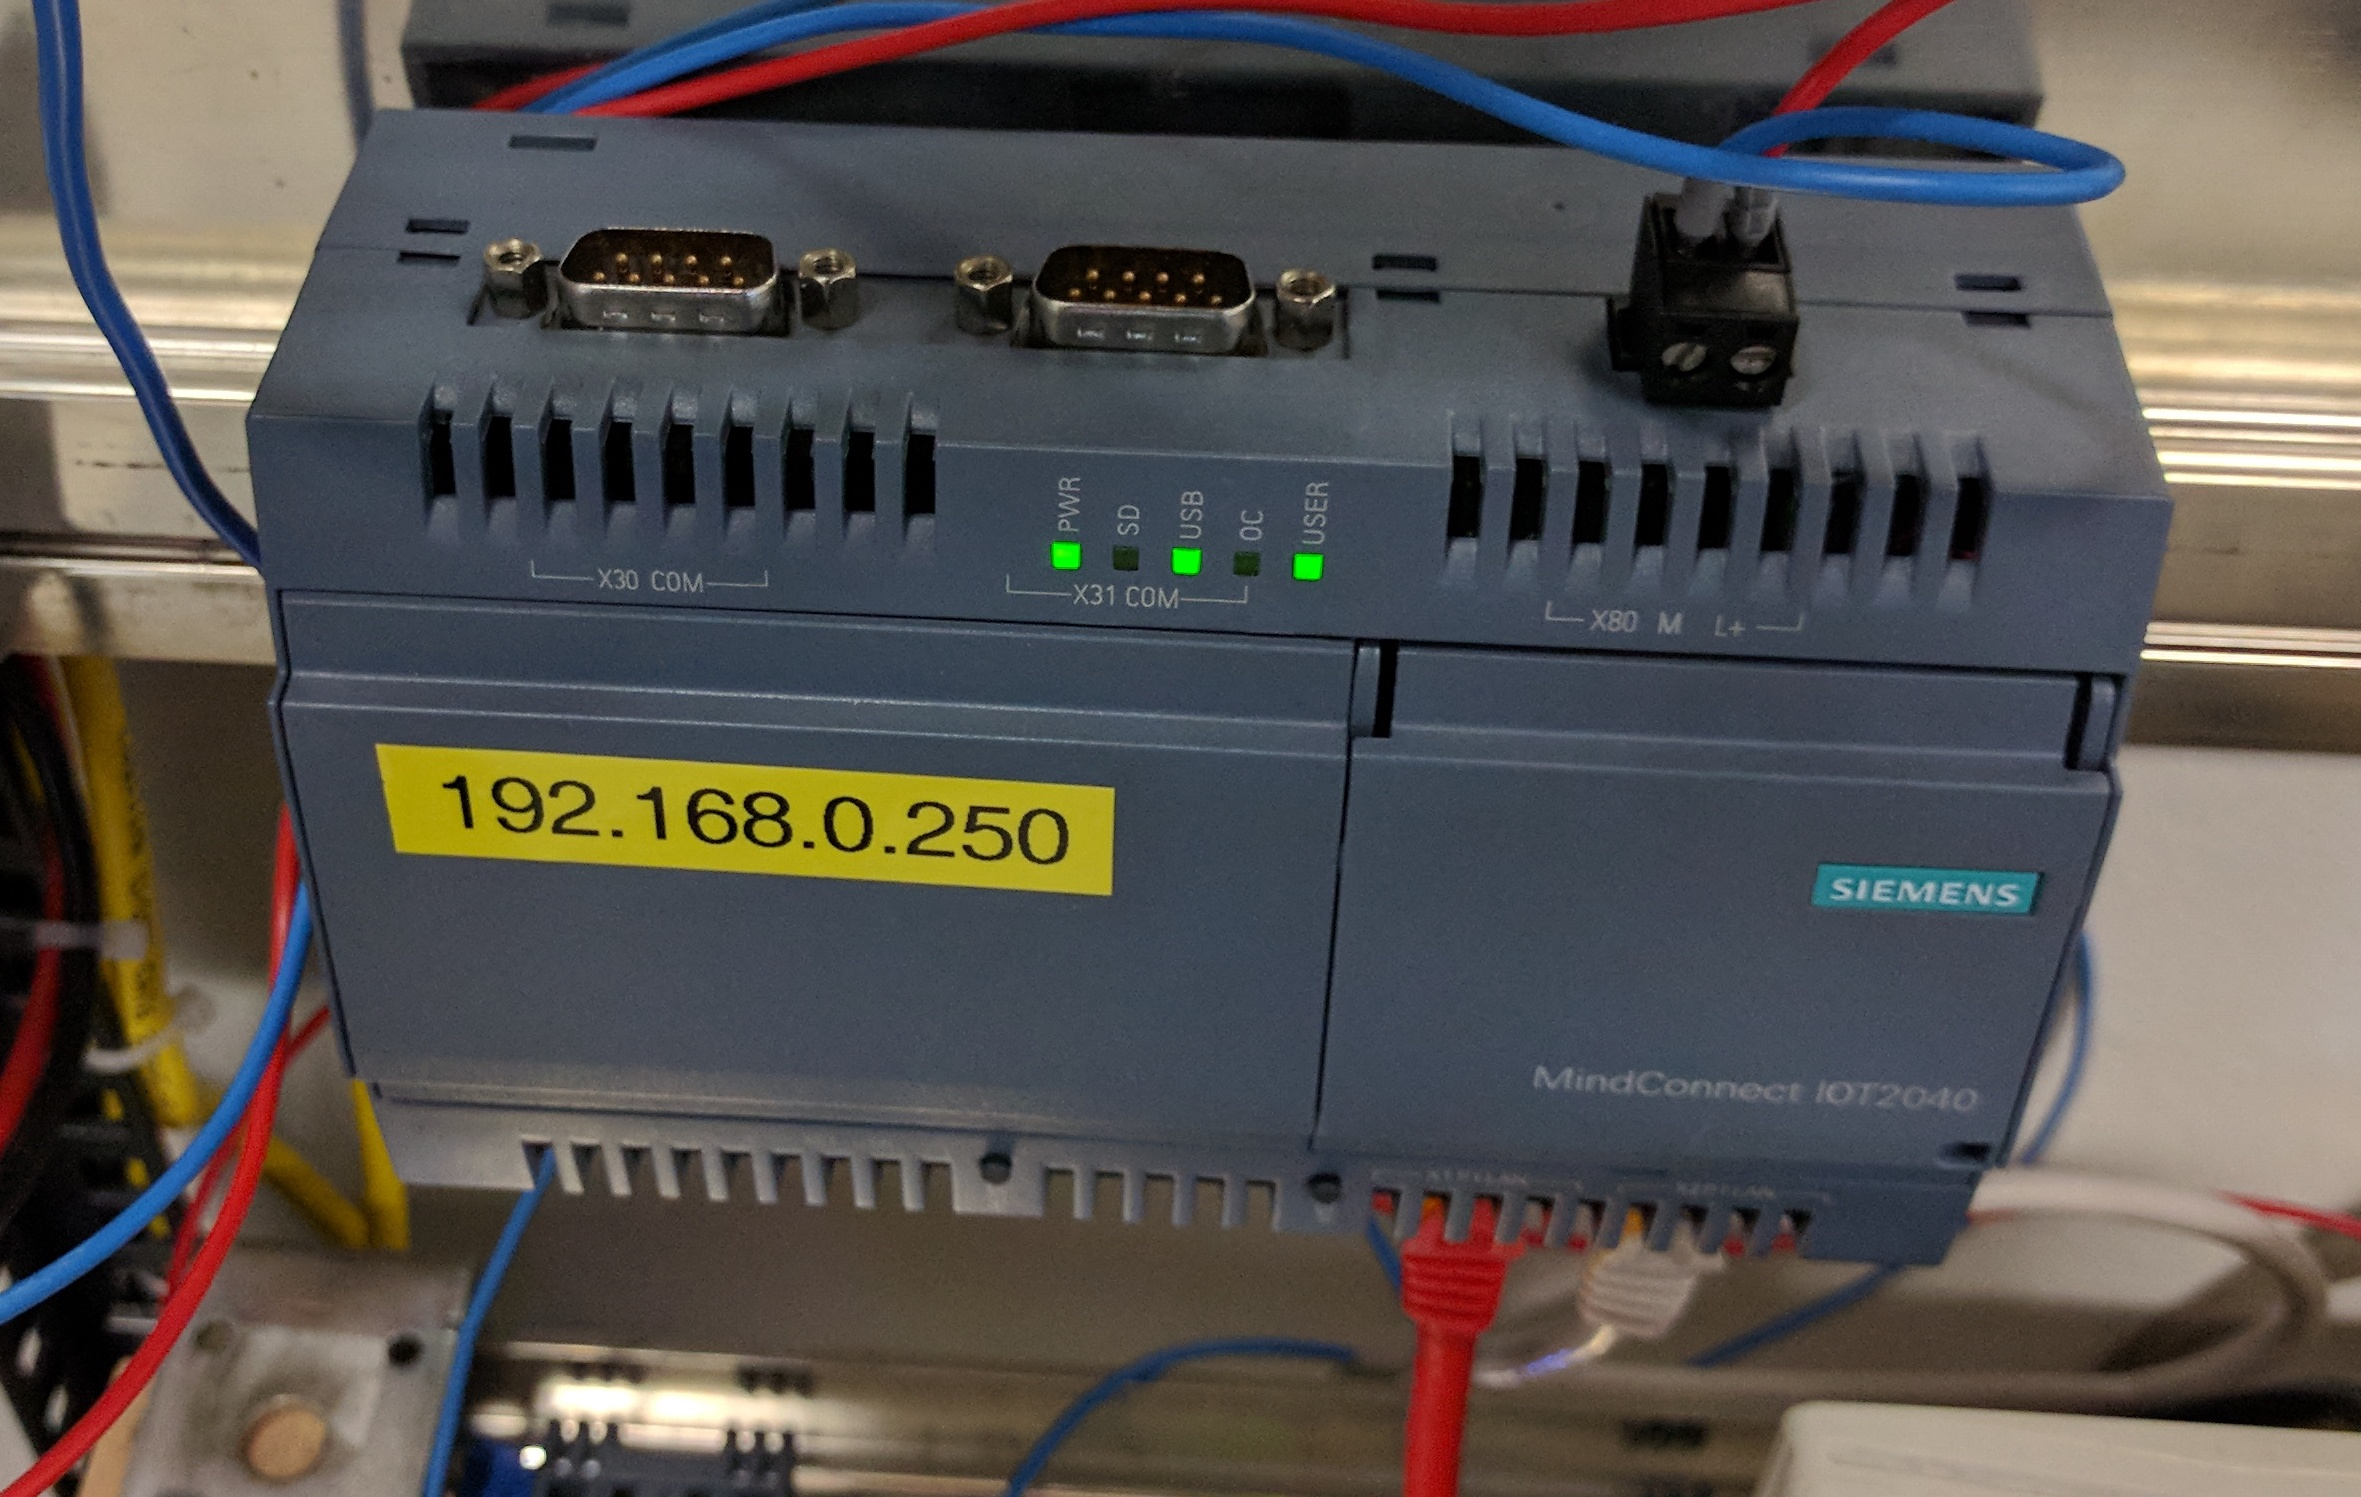
\includegraphics[width=0.45\textwidth]{MCIoT2040Foto.jpg}
\\
MindConnect Nano & MindConnect IoT2040
\end{tabular}
\caption{Siemens MindConnect Elemente \cite{SiemensMSIntroduction}.}
\label{fig:MSConnect}
\end{figure}
\vspace{\baselineskip}

\begin{itemize}
\item \ac{MCN}:\\
\ac{MCN} ist ein vorkonfigurierter Industrie-PC mit Verbindung zu MindSphere. Das Gerät unterstützt zur Datensammlung verschiedene Protokolle -- wie z.B. (OPC UA und S7 300/400). Die Datenübertragung erfolgt verschlüsselt und über eine sichere Internetverbindung. \ac{MCN} ist ausschließlich in Verbindung mit Siemens-Geräten verwendbar.

\item \ac{IoT2040}:\\
\ac{IoT2040} ist die kostengünstigere Alternative zu \ac{MCN}. Im Vergleich zu \ac{MCN} ist das \ac{IoT2040} kompakter und eher für kleinere Anlagen geeignet. Es unterstützt dieselben Protokolle wie \ac{MCN} und ist ebenfalls ausschließlich in Verbindung mit Siemens-Geräten verwendbar.
\end{itemize}
\vspace{\baselineskip}

Zusätzlich zu den physischen Geräten gibt es noch zwei weitere Möglichkeiten, Daten in die MindSphere Cloud zu laden:
\vspace{\baselineskip}

\begin{itemize}
\item MindConnect FB1500:\\
MindConnect FB1500 ist eine Siemens Totally Integrated Automation (TIA) Portal STEP7 Bibliothek, um die Funktionalität der Siemens S7-1500 \acs{SPS} zu erweitern. Diese Bibliothek unterstützt die verschlüsselte Übertragung von \acs{SPS}-Daten in die MindSphere Cloud. Die Konfiguration des Datenmodells erfolgt in STEP7 (TIA Portal V14). Zusätzliche Hardware ist nicht erforderlich.

\item MindConnect LIB:\\
MindConnect LIB ist ein Software Entwicklungssystem, welches die Programmierung gegen die Schnittstellen von MindSphere erlaubt. Das Kernstück der MindConnect LIB besteht aus einer C-basierten Software-Bibliothek. MindConnect LIB ist geräteunabhängig und sowohl in Verbindung mit Siemens-Geräten als auch Geräten von Drittanbietern verwendbar.
\end{itemize}
\vspace{\baselineskip}

Eine Gegenüberstellung der einzelnen MindConnect Geräte in Bezug auf Pufferspeichergröße, unterstützte Protokolle, Lese- und Transferzyklen ist in Tabelle \ref{tab:mindConnect} ersichtlich.

\begin{table}[H]
	\caption{Gegenüberstellung der einzelnen MindConnect Geräte \cite{SiemensWhitepaper}.} 		\label{tab:mindConnect}
	\centering
	\setlength{\tabcolsep}{5mm} % separator between columns 
	\def\arraystretch{1.25} % vertical stretch factor 
	\begin{tabular}{r|ccc}
 	  % \hline
   		& \emph{MC Nano} & \emph{IoT2040} & \emph{FB1500} \\
    	\hline
    	%\hline
    	Lokaler Pufferspeicher & 500MB & 500MB & 500MB \\
    	%\hline
    	Unterstützte Protokolle & S7/OPC UA & S7/OPC UA & S7-1500 \\
    	%\hline
   	 	max. Datenlesezyklus\\(Datenpunkte/Sek.) & 250 & 30   & 110 \\
    	%\hline
        min. Datentransferzykluszeit\\(in Sek.) & 10 & 10   & 10 \\
    	%\hline
  	\end{tabular}
\end{table}

\subsubsection{MindSphere Cloud}
Auf der Ebene 2 -- Plattform -- befindet sich die \textit{MindSphere-Cloud-Infrastruktur}. Derzeit wird die Cloud-Infrastruktur von SAP Cloud Foundry\footnote{SAP Cloud Foundry: https://cloudplatform.sap.com/index.html} als offene Plattform mit \ac{PaaS} zur Verfügung gestellt. Für die Zukunft ist eine Zusammenarbeit mit weiteren großen Partnern wie Amazon Web Services\footnote{Amazon Web Services: https://aws.amazon.com/}, AtoS\footnote{AtoS: https://atos.net/de-at/austria} und Microsoft Azure\footnote{Microsoft Azure: https://azure.microsoft.com/de-de/} geplant \parencite{SiemensMSIntroduction}. 

\subsubsection{MindApps}
Darüber befindet sich auf Ebene 3 -- Applikationen -- die \textit{MindApps} -Applikationsschicht. Industrielle Applikationen werden hier entwickelt. Mit Hilfe dieser Webapplikationen können die Daten einerseits dargestellt und andererseits analytisch ausgewertet werden. 

MindApps werden auf Basis von HTML5 entwickelt und daher in einem Browser betrieben.

\subsection{Stärken von MindSphere}
Durch die Cloud-Infrastruktur basierend auf SAP Cloud Foundry wird eine gute Skalierbarkeit erreicht \parencite{SiemensMSIntroduction,SiemensWhitepaper}. Das bedeutet, dass sowohl kleine Datenmengen (wenige MB) als auch Big Data verarbeitet werden können. Im Bezug auf Datenmenge ist es möglich schnell -- auch temporär-- auf- oder abzuskalieren. 
\vspace{\baselineskip}

Weitere Vorteile:
\begin{itemize}
\item Hohe Sicherheitsstandards:
MindConnect Elemente basieren auf \ac{ICS}-Sicherheit, orientiert an Industrie Standard IEC 62443\footnote{IEC 62443: Industrial communication networks – Network and system security} und ISO 27001\footnote{ISO 27001: Information technology – Security techniques – Information security management systems – Requirements} \parencite{SiemensMSMCSecurity}. Aus Sicherheitsgründen ist es nur möglich, Daten über die MindConnect Elemente aus den Assets zu extrahieren und nicht Daten in die Assets einzuspielen. Die Datenübertragung erfolgt mit mindestens 256 Bit SSL/TLS-Verschlüsselung.
\item Hohe Anzahl an installierten Geräten:
Derzeit gibt es im Umfeld Siemens ca. 30 Millionen Automatisierungssysteme, ca. 70 Millionen Smart Meter und ca. 800.000 vernetzte Produkte, welche potentiell mit MindSphere verbunden werden können.
\item Digitalisierung:
Durch die Möglichkeit eines digitalen Zwillings lassen sich optimierte Simulation und Engineering realisieren.
\item Einfache Anbindung:
Das Plug-and-Play-System bei der Installation der MindConnect Elemente ermöglicht eine schnelle Anbindung der Assets. 
\item REST:
Die Kommunikation ist auf Grund einer HTTP-basierter RESTfull API Firewall- und Entwickler-freundlich.  
\end{itemize}

\subsection{Technische Einschränkungen}
Folgende technische Einschränkungen existieren derzeit \parencite{SiemensMSTraining}: 

\begin{itemize}
	\item \acl{MCN}:
    	\begin{itemize}
			\item Es können maximal 250 Float-Werte alle fünf Sekunden gelesen werden.
			\item Es können maximal 10 Variablen jede Sekunde gelesen werden.
			\item Maximal drei S7-\ac{SPS} können mit einem MCN verbunden werden. 
			\item Maximal acht OPC UA Server können mit einem MCN verbunden werden. 
		\end{itemize}
  	\item \ac{IoT2040}:
        \begin{itemize}
			\item Das minimale Datenübertragungs-Intervall beträgt 15 Sekunden.
			\item Es können maximal 30 Float-Werte alle 15 Sekunden gelesen werden.
			\item Maximal drei S7 können mit einem IoT2040 verbunden werden.
			\item Maximal acht OPC UA Server können mit einem IoT2040 verbunden werden.
		\end{itemize}    
  	\item FB1500:
        \begin{itemize}
			\item Es können maximal 250 Float-Werte pro Sekunde gelesen werden.
			\item Es können maximal 10 Variablen jede Sekunde gelesen werden.
			\item Die Konfiguration kann nur per TIA Portal geändert werden.
		\end{itemize}
     \item Konfigurations- bzw. Kommissionierungs-Restriktionen:
         \begin{itemize}
			\item Nach dem Anlegen können Aspects deaktiviert jedoch nicht gelöscht werden.
			\item Es sind nur maximal 200 Endkunden pro Mieter möglich.
		\end{itemize}
\end{itemize}

\subsection{Überblick über das MindSphere-Preismodell}
Siemens AG verwendet ein Pay-per-use-Preismodell. Bei der Verwendung von MindSphere fallen Kosten in folgenden Bereichen an (siehe Abb.~\ref{fig:PriceModel}):

\begin{itemize}
	\item Investition MindConnect:\\
    Für die Hardwarekomponenten \ac{MCN} und \ac{IoT2040} ist pro Gerät eine einmalige Gebühr zu entrichten. Bei den MindSphere-Varianten mit FB1500 und MindConnect LIB fallen keine Investitionsgebühren an.    	
  	\item Monatsgebühr MindAccess:\\
    Um Daten in die MindSphere Cloud speichern bzw. Daten wieder abgreifen zu können, ist eine Berechtigung mittels Zugangskonto erforderlich. Bei diesen Zungangskontos gibt es zwei Arten -- Benutzer- und Entwicklerkonto. Je nach Kontoart und den damit verbundenen Berechtigungen fallen monatliche Gebühren an.
  	\item Monatsgebühr Datenmodell:\\
    Die monatliche Gebühr für die Datenübertragung und Datenspeicherung wird für jeden Kunden nach dem jeweiligen Bedarf abhängig von der Anzahl der Datenpunkte, dem Datentyp der Messdaten, dem Lesezyklus und der Anzahl der Assets berechnet. 
\end{itemize}

\begin{figure}[H]
\centering
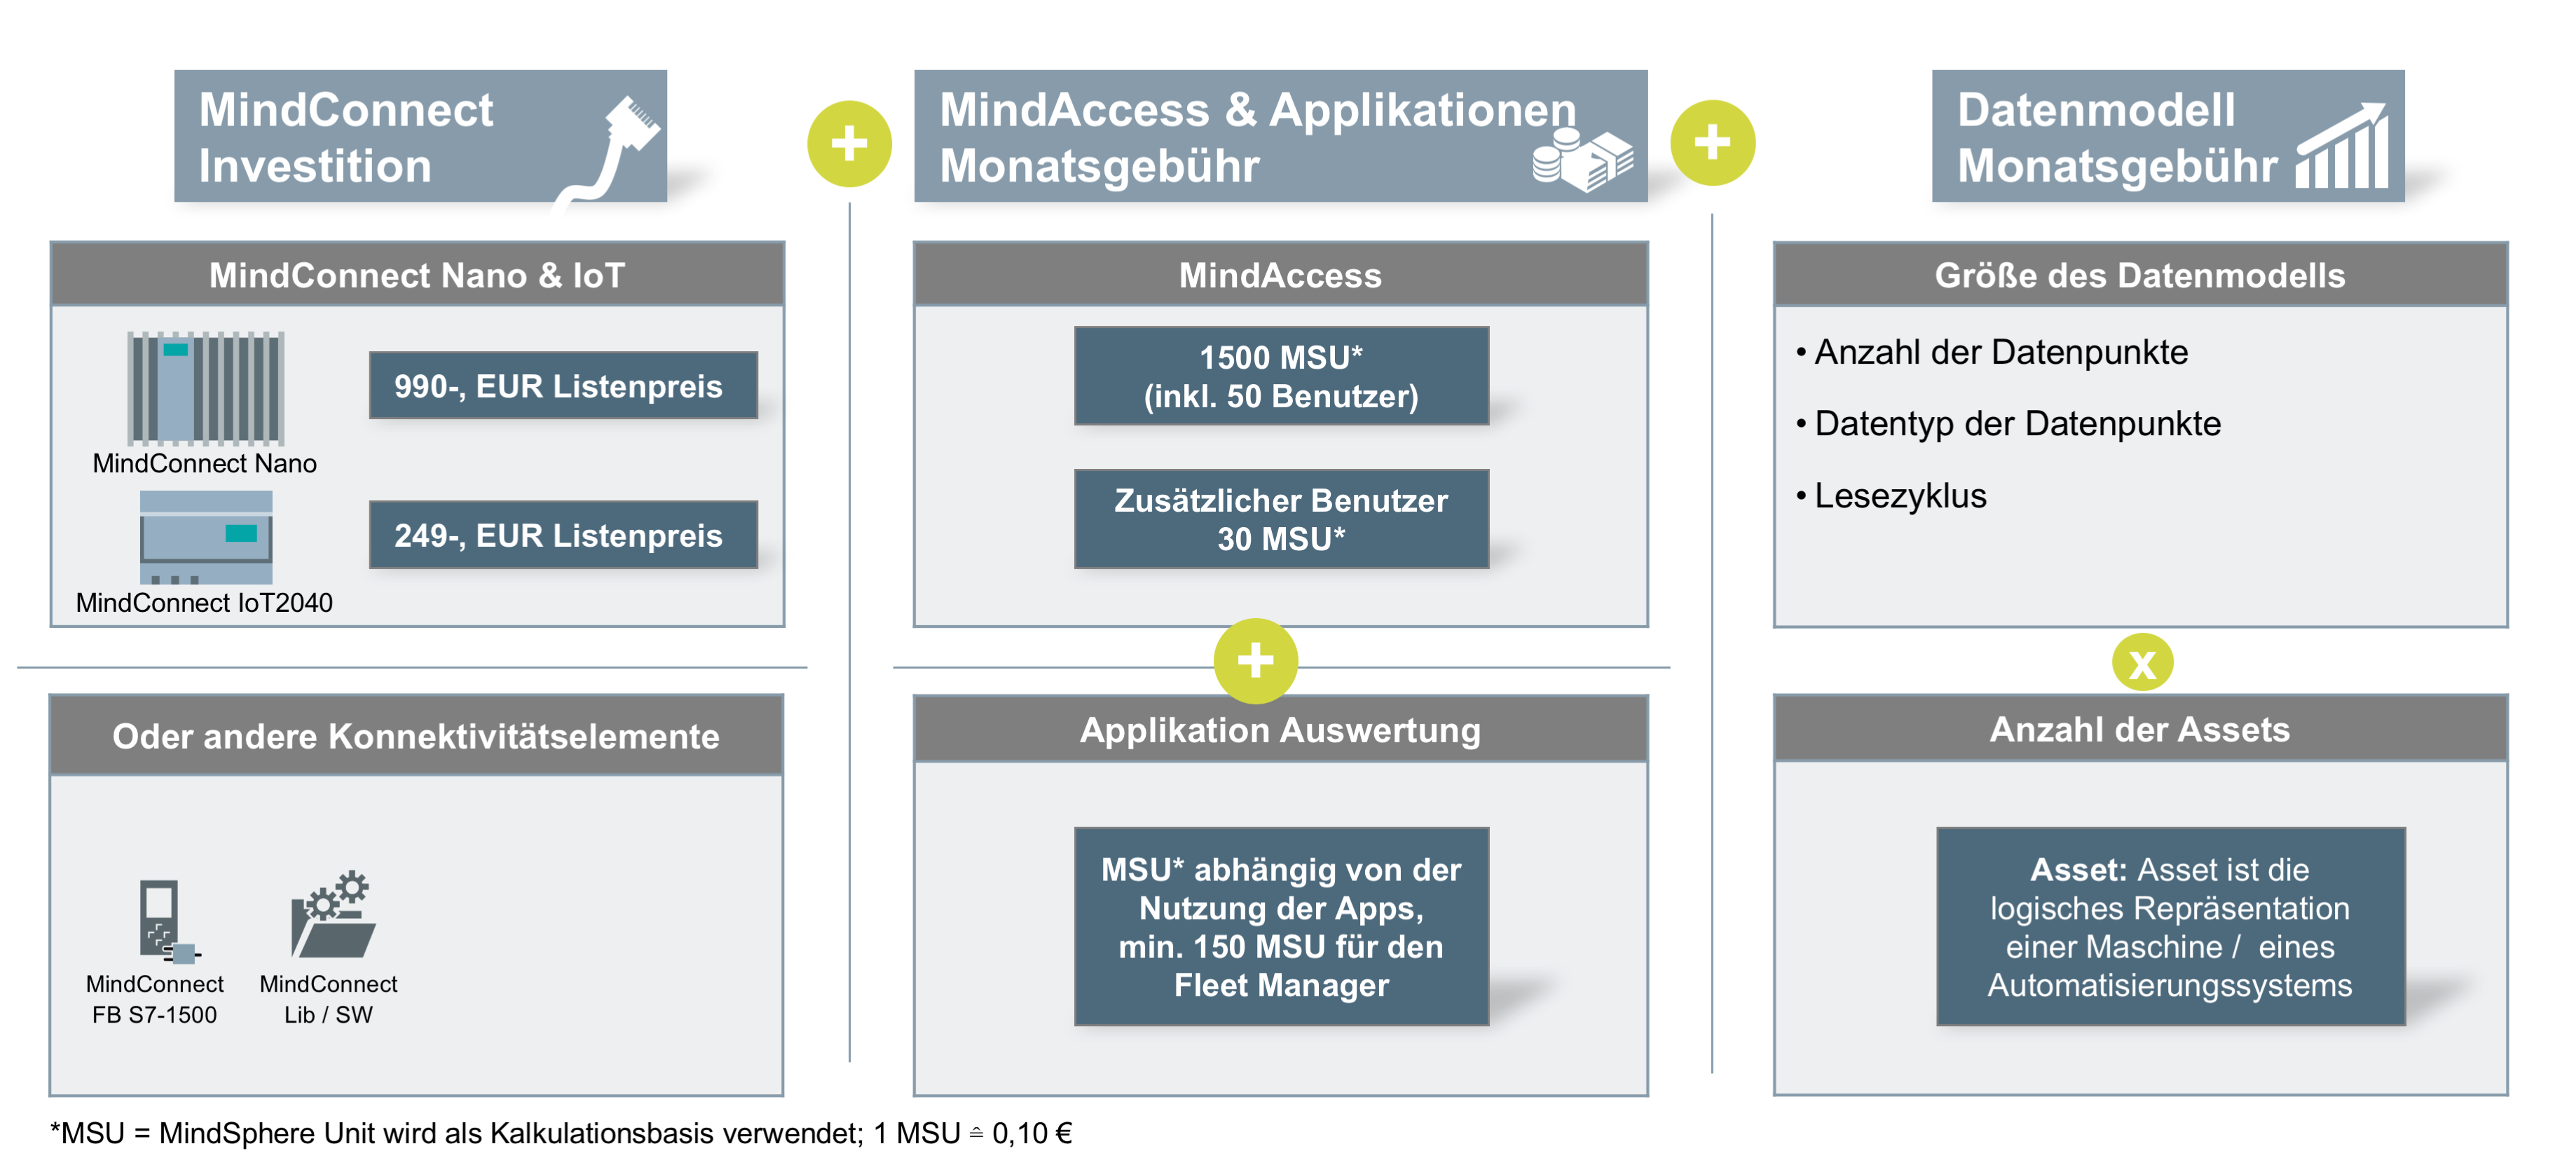
\includegraphics[width=1\textwidth]{PriceModel_1.png} 
\caption{Überblick über das MindSphere-Preismodell (vgl. \cite{SiemensMSIntroduction}).}
\label{fig:PriceModel}
\end{figure}
















\chapter{Realisierung}
\label{cha:realisierung}

\section{System-Architektur}
TODO

Die System-Architektur MindSphere ist wie in Skizze ~\ref{fig:MSSystemArchitektur} aufgebaut:

\begin{figure} [H]
\centering
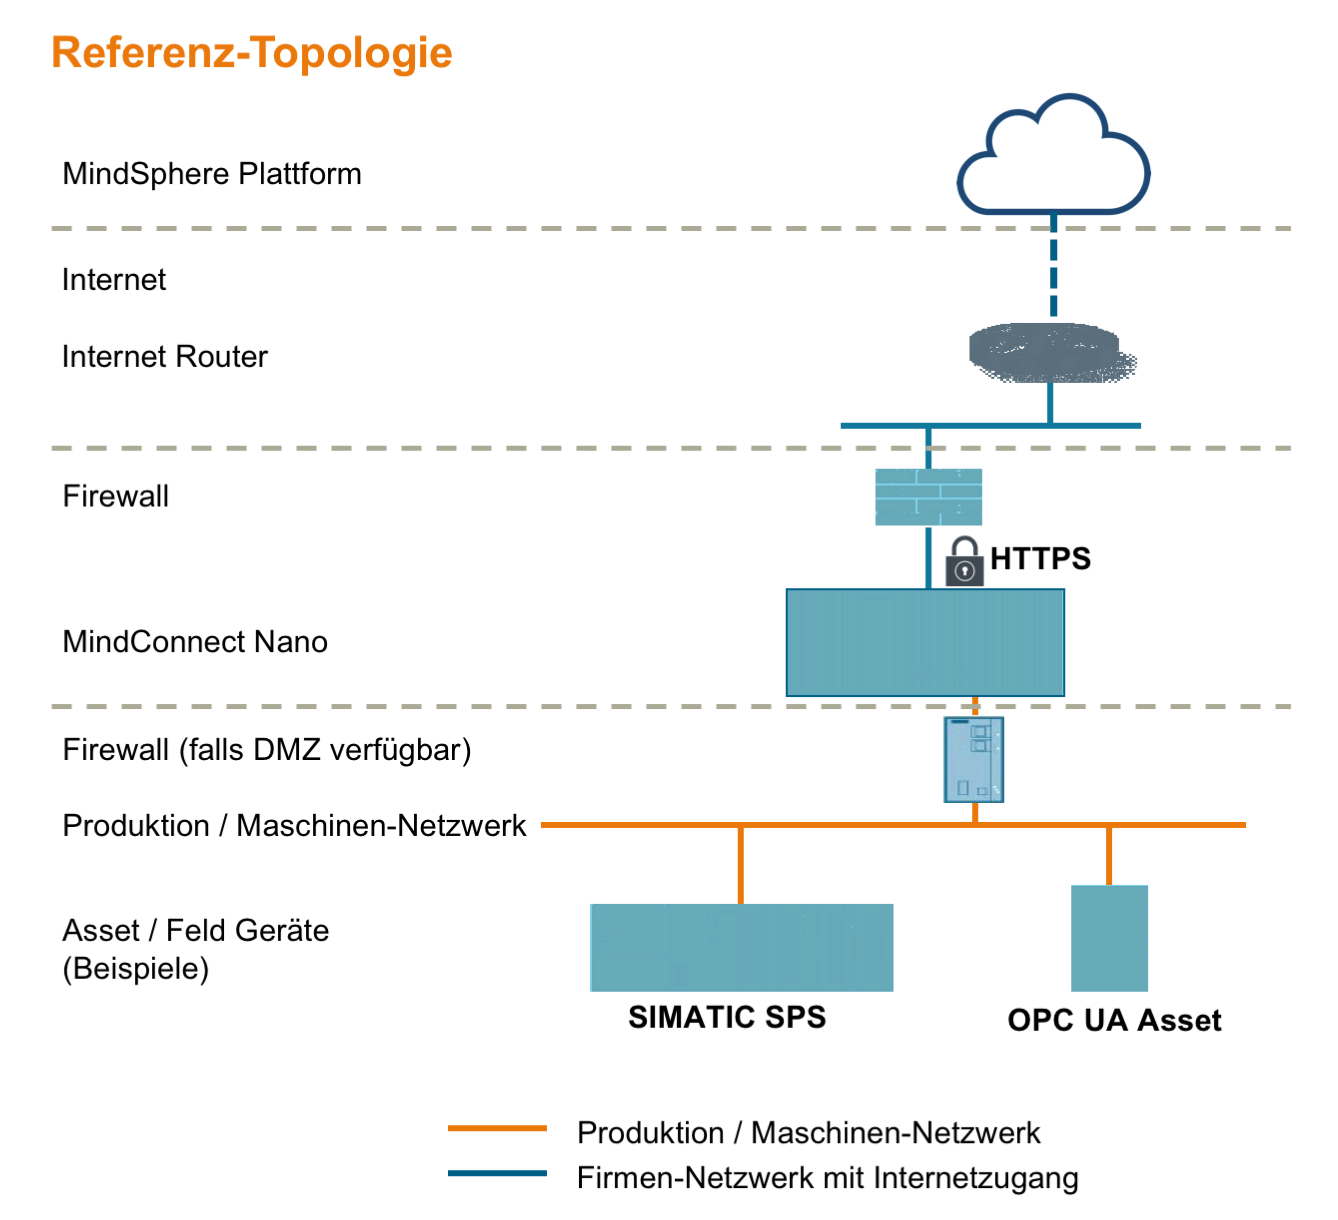
\includegraphics[width=0.8\textwidth]{MSArchitektur.png} 
\caption{Systemskizze der Architektur von MindSphere (vgl. \cite{SiemensMSMCSecurity}).}
\label{fig:MSSystemArchitektur}
\end{figure}

Auf der untersten Ebene im Produktions- bzw. Maschinen-Netzwerk befinden sich die \ac{SPS} mit optional vorgeschaltetem Router, falls das System über eine \ac{DMZ} verfügt. Das integrierte MindConnect Element wird zwischen Maschinen-Netzwerk und Firmen-Netzwerk mit Internetzugang eingebunden. Über eine Firewall und einen Router verbindet sich das MindConnect Element mit der MindSphere-Cloud. Wesentlich ist dabei, dass Daten ausschließlich von den Assets gesammelt und in die Cloud transferiert werden, jedoch der umgekehrte Weg aus Sicherheitsgründen nicht ermöglicht wird.

\subsection{Voraussetzungen für MindSphere}
TODO

\subsection{Arbeiten mit MindSphere}

\subsubsection{Einbinden von MindSphere}
Um MindSphere in ein bestehendes System einzubinden, müssen folgende 3 Schritte durchgeführt werden (siehe Abb.~\ref{fig:MSEinbinden}):

\begin{enumerate}
\item MindSphere Konto anlegen und MindConnect Element integrieren
\item Konfiguration der Datenakquisition
\item System starten
\end{enumerate}

\begin{figure}[H]
\centering
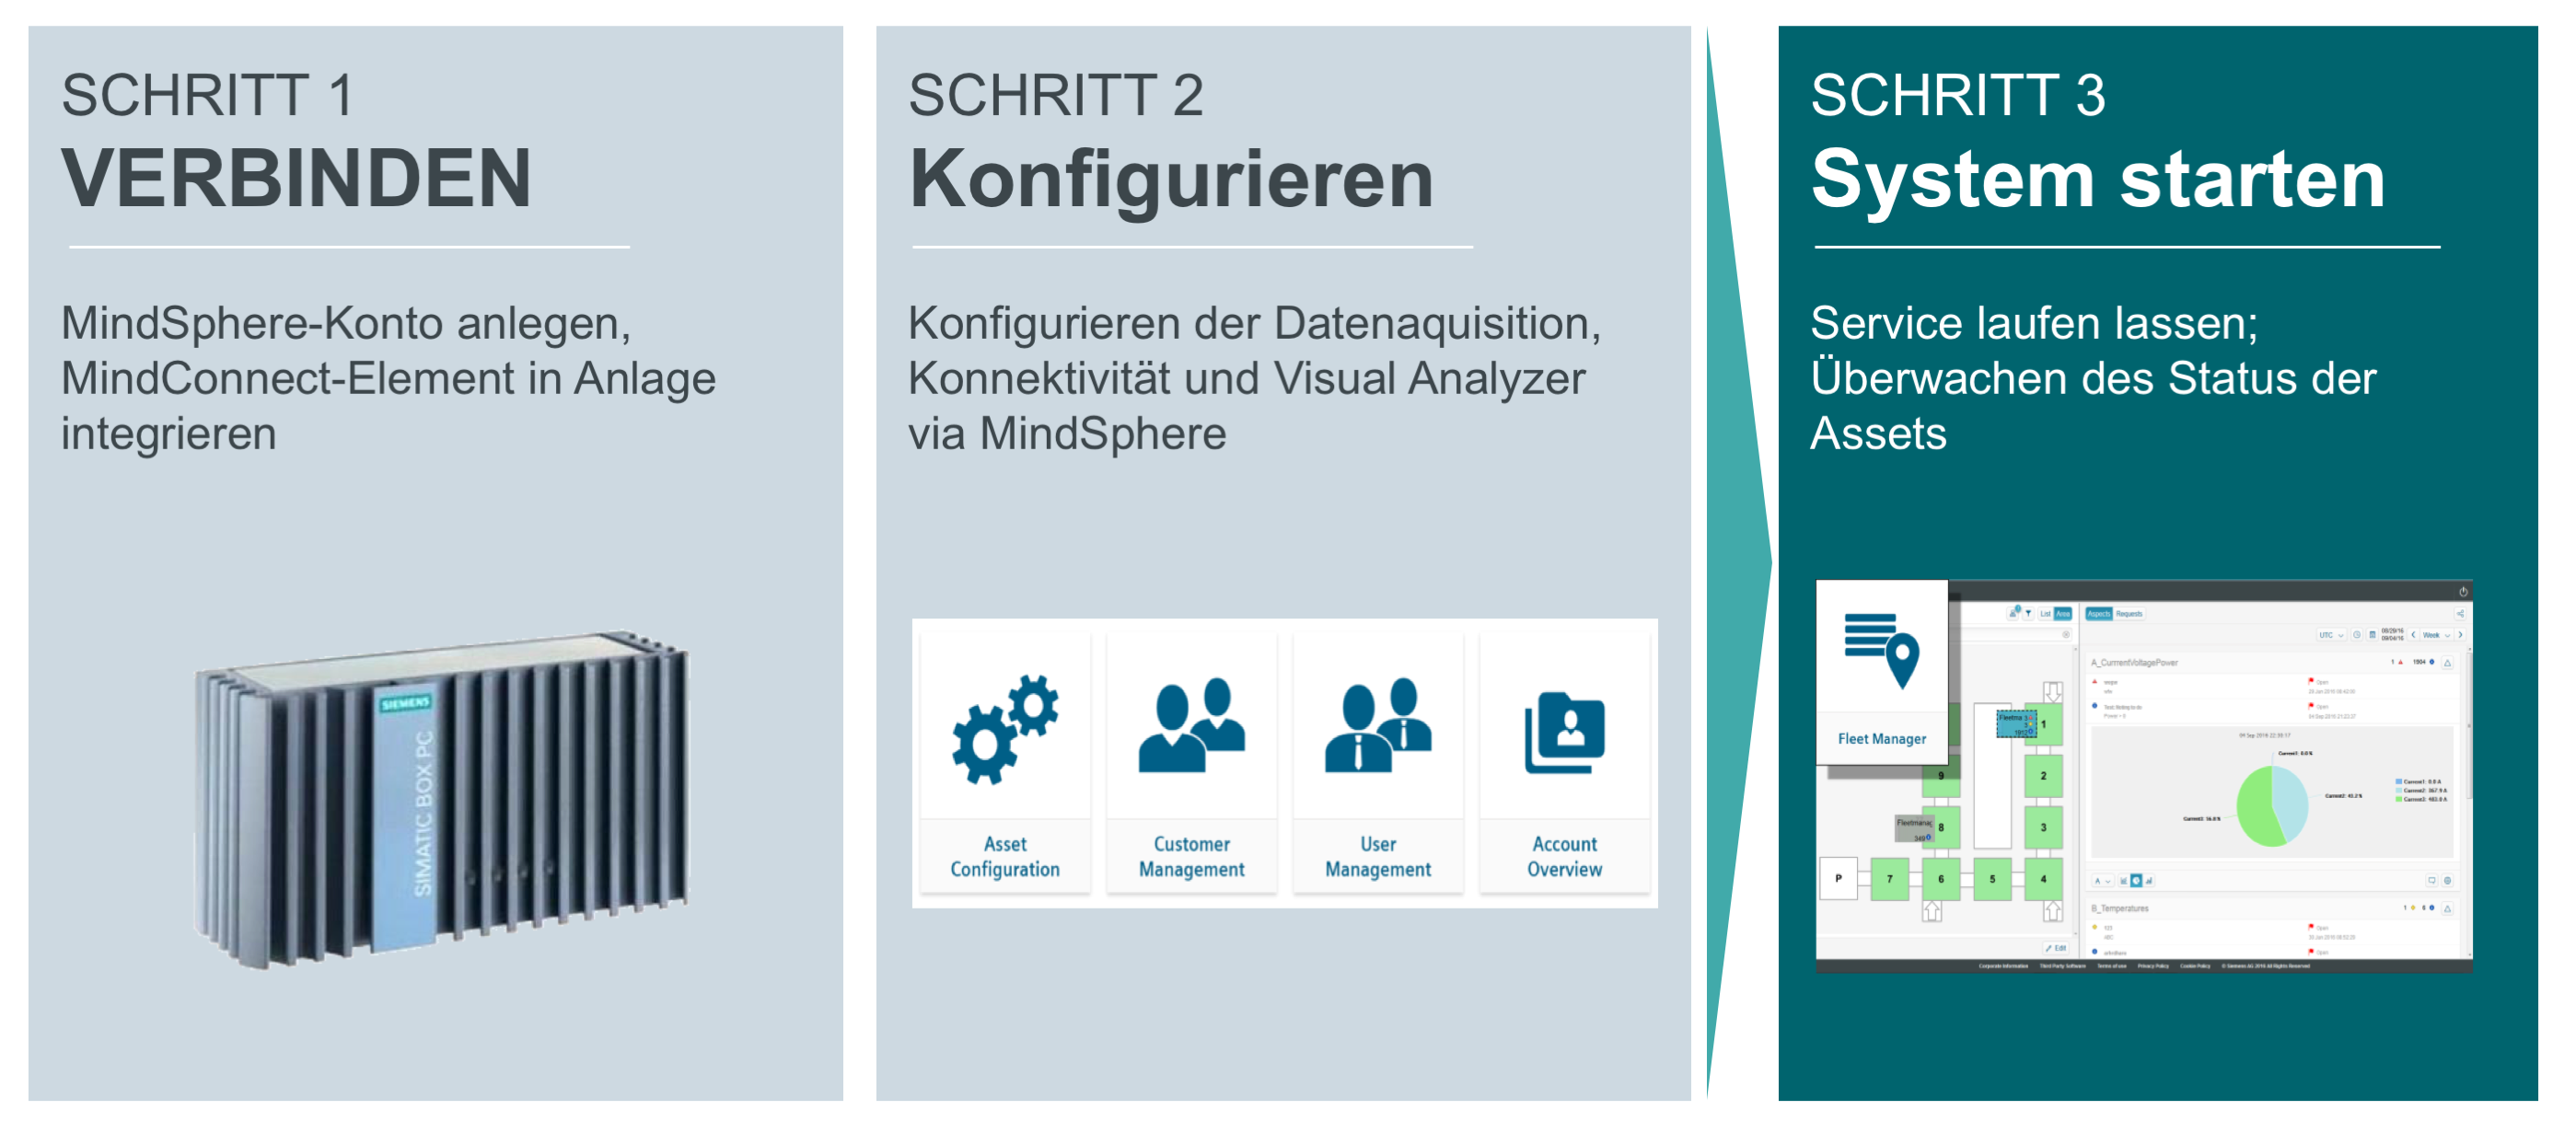
\includegraphics[width=1\textwidth]{MSEinbinden.png} 
\caption{Einbinden von MindSphere in bestehendes System (vgl. \cite{SiemensMSIntroduction}).}
\label{fig:MSEinbinden}
\end{figure}

\textit{Schritt 1}: Als erstes muss ein MindSphere Konto angelegt werden. Dabei gibt es die Unterscheidung zwischen Benutzerkonto (MindAccess User) und Entwicklerkonto (MindAccess Developer). Das Benutzerkonto erlaubt den Zugang zu den eigenen Daten im MindSphere-Ökosystem und die Benutzung der bereit gestellten MindApps. Inkludiert sind dabei zusätzlich 50 Benutzer (Endkunden), welche der MindAccess-Benutzer (Mieter) hinzufügen kann. 

Gegenüber einem Benutzerkonto können mit einem Entwicklerkonto auch Applikationen entwickelt bzw. verändert werden. 

Innerhalb des Entwicklerkontos werden wiederum drei verschiedene Konten angeboten: in den Größen S, M und L.
Eine Gegenüberstellung der Berechtigungen je nach Entwicklerkonto-Größe in Bezug auf Anzahl der EntwicklerInnenlizenzen, Anzahl der BenutzerInnen im Produktionsbereich, dem Test- und Entwicklungsspeicher und dem Speicher für Produktion ist in Tabelle \ref{tab:mindAccessDeveloper} ersichtlich.

\begin{table}[H]
	\caption{Gegenüberstellung der verschiedenen MindAccess Developer Konten (vgl. \cite{SiemensMindAccessDeveloper}).} 		\label{tab:mindAccessDeveloper}
	\centering
	\setlength{\tabcolsep}{5mm} % separator between columns 
	\def\arraystretch{1.25} % vertical stretch factor 
	\begin{tabular}{r|ccc}
 	  % \hline
   		& \emph{Größe S} & \emph{Größe M} & \emph{Größe L} \\
    	\hline
    	%\hline
    	Anzahl der EntwicklerInnen & 5 & 10 &  20\\
    	%\hline
        Anzahl der BenutzerInnen\\im Produktionsbereich & -- & 50 &  100\\
    	%\hline
   	 	Test- und Entwicklungsspeicher (RAM) & 8GB & 16GB   & 32GB \\
    	%\hline
        Speicher für Produktion (RAM) & -- & 16GB   & 32GB \\
    	%\hline
  	\end{tabular}
\end{table}





\textit{Schritt 2}: Die Datenaquisition, Konnektivität und Visual Analyzer werden im MindConnect Element via MindSphere konfiguriert.

\textit{Schritt 3}: Das System wird gestartet und läuft. Die gewünschten Daten werden gesammelt.



% marketplace geplant aber noch nicht realisiert.
% Apps derzeit in Java und Java Script
% Apps laufen in Cloud (Backend
% Derzeit 2 Apps: Fleet Manager und ManageMyMachines




\section{Architektur und Design}
TODO
Software (stat.Klassendiagramm, Ablaufdiagramm)

\section{Ausgewählte Implementierungsaspekte}
TODO


\section{Nicht-funktionale Merkmale}
TODO








\chapter{Ergebnisse und Diskussion}
\label{cha:ergebnisse}
TODO

\section{Vorschläge für künftige Weiterentwicklungen}

\chapter{Zusammenfassung und Ausblick}
\label{cha:zusammenfassung}
TODO


















%%%----------------------------------------------------------
\appendix                                            % Anhang 
%%%----------------------------------------------------------

\chapter{Abkürzungsverzeichnis}
\label{app:Abkürzungsverzeichnis}

\begin{acronym}[SCADA]
 \acro{AR}{Augmented Reality}
 \acro{AWS}{Amazon Web Services}
 \acro{BYOD}{Bring your own device}
 \acro{BYOC}{Bring your own cloud}
 \acro{CAD}{Computer-Aided Design} 
 \acro{CAM}{Computer-Aided Manufacturing}
 \acro{CAN}{Controller Area Network}
 \acro{CIM}{Computer Integrated Manufacturing}
 \acro{CPS}{Cyber Physical System}
 \acro{DMZ}{Demilitarisierte Zone}
 \acro{ICS}{Industrial Control System} 
 \acro{D2D}{Device-to-Device}
 \acro{IaaS}{Infrastructure as a Service}
 \acro{IoE}{Internet of Everything}
 \acro{IoT}{Internet of Things}
 \acro{IoT2040}{MindConnect IoT2040}
 \acro{IIoT}{Industrial Internet of Things}
 \acro{IKT}{Informations- und Kommuntikationstechnik}
 \acro{IT}{Informationstechnologie}
 \acro{M2D}{Machine-to-Device}
 \acro{M2M}{Machine-to-Machine}
 \acro{M2P}{Machine-to-People}
 \acro{MCN}{MindConnect Nano}
 \acro{MDE}{Maschinendatenerfassung}
 \acro{MES}{Manufactoring Execution System}
 \acro{NIST}{National Institute of Standards and Technology}
 \acro{OT}{Operational Technology}
 \acro{NFV}{Network Functionality Virtualization}
 \acro{P2P}{People-to-People}
 \acro{PaaS}{Platform as a Service}
 \acro{PDM}{Product Data Management}
 \acro{PLC}{Programmable Logic Controller}
 \acro{PLCs}{Programmable Logic Controller}
 \acro{PLM}{Product Lifecycle Management}
 \acro{PPM}{Predective and Preventive Maintenance} 
 \acro{PPS}{Produktionsplanungs- und Steuerungssystem} 
 \acro{RFID}{Radio-Frequency Identification}
 \acro{RTU}{Remote Terminal Units}
 \acro{RTU}{Remote Terminal Units}
 \acro{SaaS}{Software as a Service}
 \acro{SPS}{speicherprogrammierbare Steuerung}
 \acro{SCADA}{Supervisory Control and Data Acquisiton System}
 \acro{SDN}{Software Defined Networks}
 \acro{SPS}{speicherprogrammierbare Steuerung}
\end{acronym}

	% Abkürzungsverzeichnis
\chapter{Inhalt der CD-ROM/DVD}
\label{app:cdrom}

\paragraph{Format:} 
		CD-ROM, Single Layer, ISO9660-Format%
\footnote{Verwenden Sie möglichst ein Standardformat, bei DVDs natürlich
eine entsprechende andere Spezifikation.}


\section{PDF-Dateien}
\begin{FileList}{/}
%\fitem{_DaBa.dvi} Gesamtdokument (DVI-File, ohne Grafiken)
\fitem{_thesis_DE.pdf} Master- oder Bachelorarbeit mit Instruktionen (Gesamtdokument)
\fitem{_praktikum.pdf} Praktikumsbericht (verkürzte Version der Bachelorarbeit) %
\end{FileList}


\section{\latex-Dateien}

\textbf{Achtung:} Die folgende Auflistung soll nur den Gebrauch dieser Vorlage erleichtern. Es ist bei einer Master- oder Bachelorarbeit \ia\ \emph{nicht} notwendig, die zugehörigen \latex-Dateien aufzulisten (wohl aber projektbezogene Dateien, Ergebnisse, Bilder, Kopien von Online-Literatur etc.)!

\begin{FileList}{/}
\fitem{_thesis_DE.tex} Master-/Bachelorarbeit (Hauptdokument) %
\fitem{_praktikum.tex} Praktikumsbericht (verkürzte Version der Bachelorarbeit) %
\fitem{references.bib} Literatur-Datenbank (BibTeX-File)
\end{FileList}

\begin{FileList}{/thesis_DE/front}
\fitem{vorwort.tex} Vorwort %
\fitem{kurzfassung.tex} Kurzfassung %
\fitem{abstract.tex} Abstract %
\end{FileList}

\begin{FileList}{/thesis_DE/chapters}
\fitem{einleitung.tex} Kapitel 1 %
\fitem{diplomschrift.tex} Kapitel 2 %
\fitem{latex.tex} Kapitel 3
\fitem{abbildungen.tex} Kapitel 4 %
\fitem{formeln.tex} Kapitel 5 %
\fitem{literatur.tex} Kapitel 6 %
\fitem{drucken.tex} Kapitel 7 %
\fitem{word.tex} Kapitel 8 %
\fitem{schluss.tex} Kapitel 9 %
\end{FileList}

\begin{FileList}{/thesis_DE/back}
\fitem{anhang_a.tex} Anhang A (Source Code) %
\fitem{anhang_b.tex} Anhang B (Inhalt CD-ROM) %
\fitem{anhang_c.tex} Anhang C (Liste der Änderungen) %
\fitem{anhang_d.tex} Anhang D (LaTeX-Quellcode) %
\fitem{messbox.tex} Messbox zur Druckkontrolle %
\end{FileList}

\section{Style/Class-Dateien}

\begin{FileList}{/}
\fitem{hgbthesis.cls} LaTeX Class-Datei für Master- und Bachelorarbeiten
\fitem{hgb.sty} LaTeX Style-Datei für alle Hagenberg-Dokumente
\fitem{hgbabbrev.sty} LaTeX Style-Datei mit Abkürzungs-Makros
\fitem{hgbbib.sty} LaTeX Style-Datei mit Bibiographie-Einstellungen
\fitem{hgbheadings.sty} LaTeX Style-Datei für Überschriften
\fitem{hgblistings.sty} LaTeX Style-Datei für Code-Umgebungen
\end{FileList}


\section{Sonstiges}

\begin{FileList}{/images}
\fitem{*.ai} Original Adobe Illustrator-Dateien %
\fitem{*.fh11} Original Macromedia Freehand-Dateien %
\fitem{*.jpg, *.png} Original Rasterbilder %
\end{FileList}
	% Inhalt der CD-ROM/DVD
%\chapter{Chronologische Liste der Änderungen}


Diese Auflistung wird nicht mehr aktualisiert.
Siehe \emph{Commits} auf \url{https://github.com/Digital-Media/HagenbergThesis}.



\begin{comment}
\begin{sloppypar}
\begin{description}
%
\item[2002/01/07]
\verb!\newfloat{program}! repariert (auch ohne Chapter). Dank an Werner Bailer!
%
\item[2002/03/06]
Copyright-Notice an internat.\ Standard angepasst. Dank an Karin Kosina!
%
\item[2002/07/28]
"`Studiengang"' $\rightarrow$ "`Diplomstudiengang"'
%
\item[2003/08/24]
Neues Macro: \verb!\Messbox{breite}{hoehe}! -- zur Kontrolle der 
Druckgröße ohne PS-Datei. Erweiterungen für Bakkalaureatsarbeiten
%
\item[2005/04/09]
Diverse Korrekturen: Captions von Tabellen nach oben gesetzt. 
\texttt{caption} auf neue Versionen adaptiert.
\texttt{subfig} wird nicht mehr verwendet
%
\item[2006/01/20]
Adaptiert zur Verwendung als Praktikumsbericht 
(2.\ Bakk.-Arbeit)
%
\item[2006/03/24]
Fehler in \verb!\erklaerung! beseitigt (Dank an David Schwingenschlögl)
%
\item[2006/04/06]
Verwendung von T1-Fontencoding zur besseren Silbentrennung bei 
Umlauten etc.
%
\item[2006/06/21]
Neu: Bachelorstudiengang / Masterstudiengang.
Literaturverweise auf Bakk-Arbeiten.
\texttt{upquote.sty} eliminiert (Problem mit TS1-Kodierung).
Verwende Komma (statt Punkt) als Trennzeichen in Dezimalzahlen.
%
\item[2006/09/14]
Anmerkungen zum Thema Plagiarismus.
%
\item[2007/07/16]
Ergänzungen für Code-Listings (listings) und Algorithmen 
(\texttt{algorithmicx}).
BiBTeX-Datei aufgeräumt, Verwendung der Literaturformate 
verbessert.
Komma (statt Punkt) als Trennzeichen in Dezimalzahlen wieder 
entfernt.
Verwendung der \texttt{ae}-Fonts eliminiert (\texttt{cm-super} Fonts müssen 
installiert sein, ab MikTeX 2.5). 
Beispiel für Ersetzung in EPS-Dateien mit \texttt{psfrag}.
%
\item[2007/10/04]
Version 5.90: Das Laden der Pakete \verb!inputenc! (Option \texttt{latin}) und 
\verb!graphicx! (Option \texttt{dvips})
aus der Hauptdatei in die \texttt{sty}-Datei übertragen; \texttt{upquote} funktioniert nun.
Paket \texttt{eurosym} ergänzt für Euro-Symbol (Anregung von Andreas 
Doubrava).
Problem mit \texttt{color}-package repariert (gerasterter PDF-Ausdruck).
Hinweise bzgl.\ Literatur ergänzt (\texttt{month}, \texttt{edition}),
BibTeX-Datei gesäubert.
Hinweis zum Einfügen von vertikalem Abstand zwischen Absätzen.
Mathematik aufgeräumt, Verwendung von \texttt{amsmath}, 
Fallunterscheidungen.
Diverse Änderungen bei Tabellen und Programmkode.
Beispiele für BibTeX-Angaben von Spezialquellen: Audio-CDs, 
Videos, Filme. Einbinden von Dateien mit \verb!\include{..}!
Neue Datei: \verb!_SimpleReport.tex! für kurze Reports (Projekte etc.).
%
\item[2007/11/11]
Version 5.91: Hinweise zur Einstellung der Output-Profile in
TexNicCenter, Inverse Search Einstellung in YAP im Anhang.
%
\item[2008/04/01]
Version 6.00beta -- kompletter Umbau!
Auslagerung der Doku\-menten-relevanten Teile in eine eigene 
\emph{class}-Datei (\texttt{hgbthesis.cls}) mit Optionen.
Die neue Style-Datei \texttt{hgb.sty} ist nun unabhängig vom 
Dokumententyp und nicht mehr kompatibel mit älteren Versionen!
Die Liste der Änderungen ist jetzt in der Datei \verb!_ChangeLog.tex!
(DIESE Datei) und diese wird im Anhang eingebunden.
Heading-Style auf Sans Serif geändert (ohne grausliche "`Caps"').
%
\item[2008/05/22]
Neue Vorlage für Technical Reports (Klasse \texttt{hgbreport.cls}).
Spracheinstellung nunmehr mit \texttt{babel}-Paket, Hauptsprache
des Dokuments kann als Option der Klasse angegeben werden.
Sprachumschaltung innerhalb des Dokuments funktioniert nun
richtig. Mit der Sprachoption \texttt{german} wird automatisch die neue deutsche 
Orthographie (\texttt{ngerman}) verwendet.
\texttt{babelbib} wird zur Formatierung des Literaturverzeichnisses
verwendet (neue BibTeX-Style-Optionen!).
Header werden nunmehr mit \texttt{fancyhdr}-Paket erzeugt.
Versionsnummerierung von \texttt{.cls} und \texttt{.sty} Files wird beendet 
(ab jetzt gilt: \emph{Datum} = \emph{Version}). 
%
\item[2008/06/10]
Neues Listing-Environment \texttt{PhpCode}; bei allen Listing-Eviron\-ments ist nun 
\texttt{mathescape=false} (kein Math-Mode nach \verb!$!). 
Bug bei Sprachumschaltung auf \texttt{ngerman} beseitigt.
%
\item[2008/08/15]
Diverse Kleinigkeiten in Literaturangaben überarbeitet (Dank an Norbert Wenzel), Spracheinstellung vereinheitlicht, Umlaute in \texttt{.bib}-Datei ersetzt.
%
\item[2008/10/15] 
Zusätzliche Hinweise zur MikTeX-Installation (Windows) sowie LaTeX unter Mac OS~X und Linux.
Liste der Abkürzungen ergänzt.%
\item[2008/11/15] 
Diverse Schreibfehler korrigiert (Dank an Silvia Fuchshuber). Hinweis auf 
\texttt{sloppypar}-Umgebung.
%
\item[2008/12/09] 
BibTeX-Tools: neuer Hinweis auf JabRef ergänzt, BibEdit entfernt (ist nicht mehr auffindbar).
%
\item[2009/02/09]
\texttt{hgb.sty}: Option "`\texttt{spaces}"' zu \texttt{url}-Package ergänzt (ermöglicht gezielten Zeilenumbruch in URLs). 
Im allgemeinen Setup für \texttt{listings}: \texttt{keepspaces=true};
Obsoletes Environment \texttt{sourcecode} deaktiviert.
Escape-Mode für \texttt{LaTeXCode}-Umgebung geändert.
\verb!_DaBa.tex!: Hinweis auf die Verwendung von \verb!\urldef! für die Angabe von URLs in Captions. \texttt{diplom} (statt \texttt{master}) als Standard-Dokumententyp in \verb!_DaBa.tex! ("`Diplomarbeit"'). Neuer Abschnitt zum Umgang mit ``Quellenangaben in Captions''.
\texttt{literatur.bib}: alle URLs (bisher in \texttt{note}-Einträgen) auf \verb!url={..}! geändert.
%
\item[2009/04/14]
Hinweis zum Einfügen einfacher Anführungszeichen ergänzt.
%
\item[2009/07/18]
Literaturangaben korrigiert und ergänzt.
%
\item[2009/11/27]
Experimentelle Version: Massive Änderungen, Umstieg auf \texttt{pdflatex}.
%
\item[2010/06/15]
Erstes Release der neuen Version mit \texttt{pdflatex}.
\item[2010/06/23]
Konflikt zwischen \texttt{pdfsync}-Package und \texttt{array}-Package (wird relativ häufig benutzt) durch \verb!\RequirePackage[novbox]{pdfsync}! behoben.
Seitenunterkante durch \verb!\flushbottom! fixiert,
variablen Absatzzwischenraum reduziert.
\item[2010/07/27]
Sprache der Erklärungsseite auf "`\texttt{german}"' fixiert (auch wenn die Hauptsprache des Dokuments  Englisch ist). %Datumsproblem - Hinweis von Philipp Winter
\item[2010/12/03]
Anmerkungen und Beispiele zum Zitieren von Gesetzestexten und Videos (Zeitangabe) ergänzt.
Hinweis auf \verb!\nolinkurl{..}! zur Angabe von Dateinamen.
\item[2011/01/29]
Einbau der Creative Commons Lizenz und entsprechender Hinweis in 
Abschnitt \ref{sec:HagenbergEinstellungen}. Neue Makros
\verb!\strictlicense!,
\verb!\cclicense! und
\verb!\license{...}!.
BibTeX-Einträge für Audio-CDs und Filme korrigiert, Beispiel für Online-Video ergänzt.
\item[2011/02/01]
Neues Makro \verb!\betreuerin{..}! zur Angabe einer (weiblichen) Betreuerin. 
%
\item[2011/06/26]
Umstellung der gesamten Literaturverwaltung auf \texttt{biblatex} mit dem Ziel, 
getrennte Abschnitte für verschiedene Kategorien von Einträgen im Quellenverzeichnis
zu ermöglichen. Die Wahl fiel auf \texttt{biblatex} (es gäbe andere Optionen), weil
damit BibTeX weiterhin nur einmal aufgerufen werden muss (und nicht für
mehrere Dateien). Damit verbunden sind allerdings massive Änderungen bei der
Syntax der BibTeX-Felder und es gibt auch mehrere neue Felder.
Aktuell sind 3 Kategorien von Quellen vorgesehen, entsprechende Änderungen in 
\nolinkurl{hgbthesis.cls}. Der klassische BibTeX-Workflow wird aktuell nicht
mehr unterstützt, die Möglichkeit einer künftigen Dok-Option ist aber 
vorgesehen. Das Literatur-Kapitel ist komplett überarbeitet, die .bib-Datei
wurde ausgemistet. Neu ist die Empfehlung zur Aufnahme von Bildquellen
in das Quellenverzeichnis, womit lange URLs in Captions (dort sind keine
Fußnoten möglich) nicht mehr notwendig sind. 
"`Persönliche Kommunikation"' als Literaturquelle entfernt (den Inhalt
von Interviews sollte man direkt im Anhang wiedergeben).
Das verwendete Bildmaterial wurde
erneuert, aktuell werden nur mehr Public Domain Bilder verwendet. 
Das Kapitel "`Hinweise für Word-Benutzer"' wurde endgültig entfernt.
\verb!\flushbottom! wieder auf \verb!\raggedbottom! geändert, um übermäßige 
Abstände zwischen Absätzen zu vermeiden.
%
\item[2012/05/10]
Hinweis auf die in Österreich bislang nicht zulässige Verwendung von "`Masterarbeit"'
entfernt, \texttt{master} ist nunmehr die Default-Dokumentenoption.
Anmerkungen zu lästigen \texttt{biblatex}-Warnungen ergänzt.
Angaben für Windows-Programmpfade auf Win7 angepasst, 
MikTeX 2.9 als Minimalerfordernis.\newline
Überflüssige Makros \verb!\damonat! und \verb!\dajahr! endgültig entfernt, statt
\verb!\abgabemonat! und \verb!\abgabejahr! ist nun das neue Makro
\verb!\abgabedatum{yyyy}{mm}{dd}! vorgesehen (unter Verwendung von internen Zählern).
Zur Formatierung von Datumsangaben wir das \texttt{datetime}-Paket verwendet.
\newline
Neue Fassung der eidesstattlichen Erklärung (inkl.\ englischer Version).\newline
PDF-Suche auf \texttt{synctex} umgestellt (\texttt{pdfsync}-Paket ist veraltet und
wird nun nicht mehr verwendet).
\newline
Die älteren Dateiversionen von \texttt{algorithmicx.sty} und \texttt{alg\-pseudo\-code.sty}
(bisher explizit beigefügt) wurden weggelassen.
\newline
Hinweis auf die \emph{Latin Modern Roman} OTF-Schriften ergänzt.
%
\item[2012/07/21]
Quellenverzeichnis: sprachabhängige Einstellung der Überschriften eingerichtet.
Titel des Quellenverzeichnisses auf "`Quellenverzeichnis"' (DE) \bzw\ "`References"' (EN) 
fixiert. Makro \verb!\MakeBibliography! hat damit keinen erforderlichen Parameter mehr.
%
\item[2012/09/17]
Wegen Änderungen im \texttt{biblatex}-package (Version 1.7, 2011/11/13) die Verwendung von
BibTeX als backend eingestellt (\texttt{backend=bibtex8}).
%
\item[2012/10/13]
Option \texttt{lowtilde} beim URL-package eingestellt (erzeugt \url{~} statt \verb!~!).
%
\item[2012/12/01]
In Abschnitt \ref{sec:FormatierungVonProgrammcode} zusätzliche Code-Umgebungen ergänzt:
\texttt{JsCode},
\texttt{PhpCode},
\texttt{HtmlCode},
\texttt{CssCode},
\texttt{XmlCode}.
%
\item[2012/12/08]
Die Code-Umgebungen in Abschn.\ \ref{sec:FormatierungVonProgrammcode} ergänzt und 
zur Verwendung von optionalen Argumenten erweitert (Hinweise in Abschnitt 
\ref{sec:FormatierungVonProgrammcode} auf die Argumente
\texttt{firstnumber=last} und \texttt{numbers=none}).
Quellenverzeichnis: den Eintragstyp \texttt{@software} für Games empfohlen und im Verzeichnis
der Kategorie \emph{avmedia} zugeordnet (Tab.~\ref{tab:BibKategorien} ergänzt). 
Game-Beispiel (von Manuel Wieser) und zusätzliche Tabelle \ref{tab:QuellenUndEintragstypen}
zur besseren Übersicht eingefügt.
%
\item[2013/05/17]
Wichtigste Änderung ist die vollständige Umstellung auf \textbf{UTF-8} unter Beibehaltung des 
\texttt{pdflatex}-Workflows. 
Damit sind zahlreiche weitere Modifikationen verbunden:
\newline
Alle Dateien (auch \texttt{.cls}, \texttt{.sty} und \texttt{.bib}) wurden auf UTF-8 konvertiert.
Damit sollte es auch keine Probleme mehr mit Umlauten und Sonderzeichen unter MacOS geben.
\newline
Die verwendete Standard-Schriftfamilie ist nun "`Latin Modern"' (\texttt{lmodern}). 
Sie ersetzt die "`CM-Super"' Schriften, mit denen es immer wieder Installationsprobleme gab.
Weiters wird jetzt das \texttt{cmap}-Paket zur besseren Such- und Kopierbarkeit von PDFs verwendet.
\newline
Das \texttt{listings}-Paket wurde durch \texttt{listingsutf8} ersetzt und für Umlaute im Quellcode adaptiert.
Eventuell sind weitere Adaptierungen notwendig.
\newline
\texttt{biber} (min.\ Version 1.5!) wird nun anstatt \texttt{bibtex} (unterstützt keine UTF-8 Dateien) verwendet,
zusammen mit \texttt{biblatex} (Version 2.5).
Die Anweisung \verb!\bibliography! wird (wieder) verwendet, allerdings nun in der Präambel,
um die \texttt{.bib}-Datei im Fileverzeichnis anzuzeigen.
\newline
Das Makro \verb!\C! (für die Menge der komplexen Zahlen \Cpx) musste wegen Problemen in der T1-Kodierung
ersetzt werden und heißt nun \verb!\Cpx!. Die Makros 
\verb!\R!, \verb!\Z!, \verb!\N!, \verb!\Q! und \verb!\Cpx! können nun auch außerhalb des Mathematik-Modus verwendet werden.
\newline
Der DVI-PS-PDF Workflow wird ab dieser Version überhaupt nicht mehr unterstützt. 
Damit ist auch das \texttt{psfrag}-Paket nicht mehr verwendbar. Entspechende Hinweise 
wurden aus dem Text entfernt.
\newline
\texttt{hyperref} wurde auf UTF-8 umgestellt.
Die grässlichen Standard-Rahmen und Farben der automatischen \texttt{hyperref}-Links wurden entfernt \bzw\ durch 
dezentere Farben ersetzt. Dadurch wird auch die Screen-Version der PDFs wieder lesbar.
\newline
Im Quellenverzeichnis wurde versuchsweise die \texttt{backref}-Option aktiviert. 
Damit werden bei allen Einträgen auch die zugehörigen Zitierstellen angegeben
(erscheint durchaus sinnvoll).
\newline
Die bisherigen Korrekturen zur \texttt{biblatex}-Formatierung wurden entfernt, 
alles arbeitet nun mit Standard-Einstellungen. Die ursächlichen Probleme in \texttt{biblatex}
scheinen in der aktuellen Version behoben zu sein.
\newline
Das Output-Profil für TeXnicCenter wurde für den neuen Workflow mit \texttt{biber} adaptiert und liegt nun in
\nolinkurl{_tc_output_profile_sumatra_utf8.tco}.
\newline
Das Windows-Script \verb!_clean.bat! wurde entfernt, da TeXnicCenter nun ein eigenes "`Clean Project"'-Kommando aufweist (in "`Build"').
\newline
Allgemeine Einstellungen zu \emph{headings} und \emph{biblatex} wurden aus der Datei \texttt{hgbthesis.cls} entfernt und in 
\texttt{hgbheadings.sty} \bzw\ \texttt{hgbbib.sty} verlagert. Diese können nun unabhängig verwendet werden (s.\ Beispiel in 
\texttt{\_TermReport.tex}).
\newline
Die Klassen-Datei \texttt{hgbtermreport.cls} wurde eliminiert, das Dokument \texttt{\_TermReport.tex} basiert nunmehr
auf der generischen LaTeX-Klasse \texttt{report}  und verwendet keine eigene \texttt{.cls} Datei mehr.
%
\item[2014/11/05]
Neu: Logo auf der Frontseite bei allen Dokumententypen. Dazu gibt es ein neues Kommando
\verb!\logofile{pic}!, wobei \verb!pic! der Name eine PDF-Datei im
Verzeichnis \verb!images/! ist. Falls \emph{kein} Logo erwünscht ist, 
kann man die Zeile einfach weglassen oder durch \verb!\logofile{}! ersetzen.
\newline
\texttt{hyperref}-Einstellungen: Einfärbung der Links wieder entfernt (\texttt{colorlinks = false}), weil beim Druck
nicht abschaltbar. Stattdessen einheitliche (dezente) Rahmen für alle Linkarten.
Zahlreiche Tippfehler eliminiert (Dank an Daniel Karzel).
\newline
Wegen eines Bugs in \texttt{biblatex 1.9} wurden die expliziten Abteilungen (\verb!\-!) in \texttt{literatur.bib}
vorübergehend entfernt (mit entsprechenden Folgen im Ergebnis). Der Bug soll in \texttt{biblatex 2.0} (derzeit noch
nicht verfügbar) behoben sein.
\newline
Package \texttt{color} auf \texttt{xcolor} geändert. In \texttt{hgb.sty} neues "`Convenience-Makro"' \verb!\etc! ergänzt.
Output-Profil für TeXnicCenter/SumatraPDF (Windows) repariert, forward/inverse Search funktioniert nun
(Datei \verb!_tc_output_profile_sumatra_utf8.tco!).
%
\item[2015/04/28]
Paket \texttt{subdepth} (zur verbesserten Platzierung von Sub- und Superscripts) 
in hgb.sty ergänzt.
%
\item[2015/07/14]
Hinweis und Abhilfe für die (nicht automatische) Silbentrennung in zusammengesetzten Wörtern.
Neu in \texttt{hgbheadings.sty}: \verb!\RequirePackage[raggedright]{titlesec}! verhindert Blocksatz
in Section-Überschriften (sehr unschön bei längeren Überschriften). 
Neu (in Abschn.~\ref{sec:GraphicOverlays}): Beispiel für die Verwendung des \texttt{overpic}-Pakets
zur Annotierung von importierten Grafiken (verwendet zudem das \texttt{pict2e}-Paket).
%
\item[2015/08/03]
Logo-Datei auf \texttt{logo.pdf} umbenannt.
\item[2015/09/17]
Anweisung \verb!\RequirePackage[utf8]{inputenc}! in die Doku\-menten\-dateien (\texttt{\_xxx.tex})
verschoben (auf Anregung von Markus Kohm: "`\ldots für die Verwendung von lualatex oder xelatex 
ist die Anweisung in hgb.sty störend, da bei diesen beiden aufgrund der nativen utf8-Unterstützung 
\texttt{inputenc} keinesfalls verwendet werden darf"').
\item[2015/09/19]
\texttt{hgb.sty} aufgeräumt.
Makros \verb!\@savesymbol! und \verb!\@restoresymbol! aus \texttt{hgb.sty} entfernt
(wurden nicht mehr verwendet; ggfs.\ Paket \texttt{savesym} als Ersatz).
Makro \verb!\optbreaknh! (optional break with no hyphen) auf \verb!\obnh! umbenannt.
Teile von \texttt{hgb.sty} in neue Dateien \texttt{hgbabbrev.sty} (div.\ Abkürzungen)
und \texttt{hgblistings.sty} (Code-Listings) verschoben.
Hintergrundtönung der Code-Listings heller (auf 5\% Grau) eingestellt.
Layout: \verb!\textfraction! auf 0.1 (statt fehlhafterweise 0.01) eingestellt.
\texttt{hgbbib.sty}: \verb!\clearpage! am Beginn des Quellenverzeichnisses entfernt
(für \texttt{article}-Template).
\item[2015/09/19]
Alle \texttt{.cls} und \texttt{.sty} Dateien sind jetzt ANSI-codiert (Header eingefügt), wie
laut CTAN-Richtlinien vorgesehen. Umlautzeichen wurden durch Makros ersetzt.
Nur \texttt{hgblistings.sty} ist weiterhin UTF-8 (wegen notwendiger literaler Umlaute).
\verb!\RequirePackage[utf8]{inputenc}! steht sonst nur mehr am Beginn
der jeweiligen (\texttt{.tex}) Haupttextdatei.
\item[2015/10/29]
Verwendung von "`In:"' im Quellenverzeichnis vor \texttt{article}-Einträgen
(Eigenart von biblatex) durch passendes Makro in \texttt{hgbbib.sty} unterbunden 
(Dank an S.\ Dreiseitl).
\item[2015/11/04]
Hinweise in Abschnitt \ref{sec:Software} auf TeXstudio unter Windows, Mac OS und Linux.
Release-Ausgabe.
\item[2015/12/08]
Source Directories neu strukturiert in \texttt{frontmatter}, \texttt{chapters}, 
\texttt{appendix}.
\item[2016/06/09]
Bibliography-Aliases für die Quellentypen
\texttt{video}, \texttt{movie}, \texttt{audio} und \texttt{software}
eingefügt (in \texttt{hgbbib.sty}) -- unterbindet Warnungen wegen
fehlender biblatex-Driver.
\item[2016/06/11]
Repository portiert auf GitHub (SourceForge eingefroren).  
Overleaf als experimentelle online LaTeX-Umgebung.
Hauptdateien umbenannt (auf \texttt{\_thesis}, \texttt{\_praktikum}, etc.).
\item[2016/09/28]
"`Numerierung"' auf "`Nummerierung"' geändert.
Code-Einbindung im Anhang repariert.
\item[2016/10/06]
In \texttt{hgb.sty}: Makros \verb!\Frametext! und \verb!\FramePic! eliminiert (ersetzt durch \verb!\fbox{...}!),
dazu \verb!\fboxsep! global auf Null gesetzt.
Hinweise auf \texttt{subfig}-Paket entfernt.
\item[2016/10/07]
In \texttt{hgbbib.sty}: Zeilenumbrüche bei URLs im Quellenverzeichnis werden an beliebigen Zeichen ermöglicht.
\end{description}
\end{sloppypar}
\end{comment}



%\section*{To Do} 
%\begin{itemize}
%\item Anhang B (CD-ROM Inhalt) überarbeiten -- ist nicht aktuell!
%\item Inkscape
%\item biblatex Bib-Driver für audio, video etc. ergänzen.
%\item Mathematik umbauen, typische Fehler stärker berücksichtigen (ua. Leerzeilen vor/nach Gleichungen).
%\item Literaturempfehlungen zum Schreiben von Diplomarbeiten
%\item Hinweise für Literatursuche (Bibliotheksverbund, CiteSeer,...)
%\end{itemize}





	% Chronologische Liste der Änderungen
%\chapter{\latex-Quellkode}
\label{app:latex}

\section*{Hauptdatei \texttt{\_thesis\_DE.tex}}

\paragraph{Anmerkung:}
Das sollte nur ein \emph{Beispiel} für die Einbindung von Quellcode
in einem Anhang sein. Der \latex-Quellkode der eigenen
Abschlussarbeit ist meist \emph{nicht} interessant genug, um ihn hier
wiederzugeben!

\begin{footnotesize}
\verbatiminput{_thesis_DE.tex}
\end{footnotesize}





	% Quelltext dieses Dokuments

%%%----------------------------------------------------------
\MakeBibliography                        % Quellenverzeichnis
%%%----------------------------------------------------------

%%% Messbox zur Druckkontrolle ------------------------------
%\chapter*{Messbox zur Druckkontrolle}



\begin{center}
{\Large --- Druckgröße kontrollieren! ---}

\bigskip

\calibrationbox{100}{50} % Angabe der Breite/Hoehe in mm

\bigskip

{\Large --- Diese Seite nach dem Druck entfernen! ---}

\end{center}



%%%----------------------------------------------------------
\end{document}
%%%----------------------------------------------------------